% The Clever Algorithms Project: http://www.CleverAlgorithms.com
% (c) Copyright 2010 Jason Brownlee. Some Rights Reserved. 
% This work is licensed under a Creative Commons Attribution-Noncommercial-Share Alike 2.5 Australia License.

% paperback.tex

\documentclass[twoside, openright]{book}
% The Clever Algorithms Project: http://www.CleverAlgorithms.com
% (c) Copyright 2013 Jason Brownlee. Some Rights Reserved. 
% This work is licensed under a Creative Commons Attribution-Noncommercial-Share Alike 2.5 Australia License.



% 
% Definitions
% 

% The main title of the book
\newcommand{\mybooktitle}{Clever Algorithms}
% The sub title of the book
\newcommand{\mybooksubtitle}{Statistical Machine Learning Recipes}
% title
\newcommand{\mybookauthor}{Jason Brownlee}
% date
\newcommand{\mybookdate}{2013}


% new macro for starting a new page and changing the style to empty
% \newpage == ends the current page. 
% \thispagestyle == works in the same manner as the \pagestyle, except that it changes the style for the current page only. 
% empty == Produces empty heads and feet - no page numbers
\newcommand{\blanknonumber}{\newpage\thispagestyle{empty}}


% 
% Packages
% 


% a replacement for fancyheadings
% http://www.ctan.org/tex-archive/macros/latex/contrib/fancyhdr/
\usepackage{fancyhdr}
\fancyhead[LO]{\slshape\nouppercase{\leftmark}}
\fancyhead[RE]{\slshape\nouppercase{\rightmark}}
\fancyhead[LE,RO]{\thepage}
\renewcommand{\headrulewidth}{0.4pt}
\renewcommand{\sectionmark}[1]{\markright{\thesection.\ #1}}
\renewcommand{\chaptermark}[1]{\markboth{\chaptername\ \thechapter.\ #1}{}}


% add an index
% http://ctan.unsw.edu.au/macros/latex/contrib/index/index.pdf
\usepackage{index} 

% Flexible and easy interface to page dimensions
% http://www.ctan.org/tex-archive/macros/latex/contrib/geometry/
% also, bigger pages by default
\usepackage[pdftex]{geometry}

% Lulu Trade Paperback
\geometry{bindingoffset=1cm, twoside, paperwidth=6in, paperheight=9in, top=.9in, bottom=.6667in, outer=0.667in}

% Supports the Text Companion fonts which provide many text symbols (such as baht, bullet, copyright, musicalnote, onequarter, section, and yen) in the TS1 encoding.
% http://www.ctan.org/tex-archive/help/Catalogue/entries/textcomp.html
% needed for listings
\usepackage{textcomp}

% http://www.maths.adelaide.edu.au/anthony.roberts/LaTeX/ltxusecol.html
% needed for listings - lots of pretty colors
\usepackage[usenames,dvipsnames]{color}

% bold in ttfamily
\usepackage{bold-extra}

% better spacing
% http://ctan.unsw.edu.au/macros/latex/contrib/microtype/microtype.pdf
\usepackage{microtype}

% code listings (lots of languages)
% http://mirror.aarnet.edu.au/pub/CTAN/macros/latex/contrib/listings/
\usepackage{listings} 
\lstset{language=r, 
	basicstyle=\footnotesize\ttfamily, 
  numbers=left, 
  numberstyle=\tiny, 
	keywordstyle=\bfseries\ttfamily,
  frame=single, 
  columns=flexible, 
  upquote=true, 
  showstringspaces=false, 
  tabsize=2, 
  captionpos=b,
  breaklines=true,
  breakatwhitespace=true}

% for ebooks, turn cross references into links
% http://www.tug.org/applications/hyperref/manual.html
\usepackage[pdftex,
	breaklinks=true,
	colorlinks=true,
	urlcolor=blue,
	linkcolor=blue,
	citecolor=blue]{hyperref}

% modifies the widths of certain columns, rather than the inter column space, to set a table with the requested total width
% http://www.cs.brown.edu/system/software/latex/doc/tabularx.pdf
\usepackage{tabularx}

% This package provide some additional commands to enhance the quality of tables in LaTeX.
% http://www.ctan.org/tex-archive/macros/latex/contrib/booktabs/
\usepackage{booktabs}

% a form of verbatim command that allows linebreaks at certain characters or combinations of characters
% http://www.tex.ac.uk/tex-archive/help/Catalogue/entries/url.html
% works well with hyperref
\usepackage{url}

% Algorithm2e is an environment for writing algorithms in LaTeX2e
% http://www.ctan.org/tex-archive/macros/latex/contrib/algorithm2e/
\usepackage[algoruled, linesnumbered, algosection]{styles/algorithm2e}

% for adding in bib for each section or chapter
% http://merkel.zoneo.net/Latex/natbib.php
\usepackage[numbers, sort&compress]{natbib}
\usepackage{styles/bibunits}

% maths
\usepackage{amsmath}
\usepackage{latexsym}

% graphics
\usepackage{graphicx}


% The Clever Algorithms Project: http://www.CleverAlgorithms.com
% (c) Copyright 2010 Jason Brownlee. Some Rights Reserved. 
% This work is licensed under a Creative Commons Attribution-Noncommercial-Share Alike 2.5 Australia License.


% Title Page


% def
\makeatletter
\def\thickhrulefill{\leavevmode \leaders \hrule height 1pt\hfill \kern \z@}
\renewcommand{\maketitle}{\begin{titlepage}%
    \let\footnotesize\small
    \let\footnoterule\relax
    \parindent \z@
    \reset@font
    \null
    \vskip 10\p@
    \hbox{\mbox{\hspace{3em}}%
      \vrule depth 0.6\textheight%
      \mbox{\hspace{2em}}
      \vbox{
        \vskip 40\p@
        \begin{flushleft}
          \Large \@author \par
        \end{flushleft}
        \vskip 70\p@
        \begin{flushleft}
          \huge \bfseries \@title \par
        \end{flushleft}
        \vfil
        }}
    \null
  \end{titlepage}%
  \setcounter{footnote}{0}%
}
\makeatother
\author{\mybookauthor}
\title{\mybooktitle\\{\large\mybooksubtitle}}
\date{\mybookdate}
\makeindex

% paperback only
\geometry{bindingoffset=1cm, twoside, paperwidth=6in, paperheight=9in, top=.9in, bottom=.6667in, outer=0.667in}

% \includeonly{f_copyright}

\begin{document}
\defaultbibliography{../workspace/bibtex}
\frontmatter
	\maketitle
	% The Clever Algorithms Project: http://www.CleverAlgorithms.com
% (c) Copyright 2010 Jason Brownlee. Some Rights Reserved. 
% This work is licensed under a Creative Commons Attribution-Noncommercial-Share Alike 2.5 Australia License.

% copyright.tex

\vspace*{\fill}
\begin{flushleft}
\begin{small}

% The Cover
\subsubsection*{Jason Brownlee, PhD}
Jason Brownlee studied Applied Science at Swinburne University in Melbourne, Australia, going on to complete a Masters in Information Technology focusing on Niching Genetic Algorithms, and a PhD in the field of Artificial Immune Systems. Jason has worked for a number of years as a Consultant and Software Engineer for a range of Corporate and Government organizations. When not writing books, Jason likes to compete in Machine Learning competitions.

% The Cover
\subsubsection*{Cover Image}
\copyright\ Copyright \mybookdate\ \mybookauthor. All Reserved. \\
\vspace{0.5cm}

% The Book
\subsubsection*{\mybooktitle: \mybooksubtitle}
\copyright\ Copyright \mybookdate\ \mybookauthor. Some Rights Reserved. \\
\vspace{0.5cm}

EDITON \\
ISBN \\
\vspace{0.5cm}

This work is licensed under a Creative Commons Attribution\--Noncommercial\--Share Alike 2.5 Australia License. \\
The full terms of the license are located online at \url{http://creativecommons.org/licenses/by-nc-sa/2.5/au/legalcode} \\
\vspace{0.5cm}

\subsubsection*{Webpage}
Source code and additional resources can be downloaded from the books companion website online at \url{http://www.CleverAlgorithms.com}

\end{small}
\end{flushleft}

		
	\cleardoublepage% The Clever Algorithms Project: http://www.CleverAlgorithms.com
% (c) Copyright 2013 Jason Brownlee. Some Rights Reserved. 
% This work is licensed under a Creative Commons Attribution-Noncommercial-Share Alike 2.5 Australia License.



\setcounter{tocdepth}{1}
\tableofcontents
	\addtocontents{toc}{\protect\markboth{Contents}{}}
	\cleardoublepage% The Clever Algorithms Project: http://www.CleverAlgorithms.com
% (c) Copyright 2013 Jason Brownlee. Some Rights Reserved. 
% This work is licensed under a Creative Commons Attribution-Noncommercial-Share Alike 2.5 Australia License.



% Foreword 
\chapter*{Foreword\markboth{Foreword}{}}
\addcontentsline{toc}{chapter}{Foreword}
The forward is not yet written.

\begin{flushright}
\vspace{0.5in}
Forward author details.
\end{flushright}

\begin{flushleft}
\vspace{0.2in}
Location \\
Date
\end{flushleft}

	\cleardoublepage% The Clever Algorithms Project: http://www.CleverAlgorithms.com
% (c) Copyright 2011 Jason Brownlee. Some Rights Reserved. 
% This work is licensed under a Creative Commons Attribution-Noncommercial-Share Alike 2.5 Australia License.


% A preface generally covers the story of how the book came into being, or how the idea for the book was developed; this is often followed by thanks and acknowledgments to people who were helpful to the author during the time of writing.
\chapter*{Preface\markboth{Preface}{}}
\addcontentsline{toc}{chapter}{Preface}

% 
% About the book
% 
\section*{About the book}
Not written yet.

\begin{flushright}
\vspace{1in}
Jason Brownlee
\end{flushright}

\begin{flushleft}
\vspace{0.2in}
Melbourne, Australia \\
2011
\end{flushleft}

	\cleardoublepage % The Clever Algorithms Project: http://www.CleverAlgorithms.com
% (c) Copyright 2013 Jason Brownlee. Some Rights Reserved. 
% This work is licensed under a Creative Commons Attribution-Noncommercial-Share Alike 2.5 Australia License.


% Acknowledgments
\chapter*{Acknowledgments\markboth{Acknowledgments}{}}
% general
This book could not have been completed without the commitment, passion, and hard work from a large group of editors and supporters.

In no particular order, thanks to: 
David Howden, 
James Montgomery, 
and
Daniel Angus.
	
\mainmatter 
	\part{Background}
		% The Clever Algorithms Project: http://www.CleverAlgorithms.com
% (c) Copyright 2010 Jason Brownlee. Some Rights Reserved. 
% This work is licensed under a Creative Commons Attribution-Noncommercial-Share Alike 2.5 Australia License.

% This is a chapter


\begin{bibunit}

% Argument and background information the user requires to read and understand the book
\chapter{Introduction}
\label{chap:intro}

Not written yet.




\section{Considerations}


\subsection{The bias-variance tradeoff}

bias - approximation is too crude
variance - overfitting training data

typically when the bias is low, variance is high, and vice-versa

each problem has a sweet-spot in this trade-off
i.e. prediction error on the training set goes down, but prediction error on the test set goes down then back up, you want the bottom of that inflection point.

this has to do with model selection - which model to use

cross validation addresses this problem - average fit over each fold gives a better idea of performance.

voting an ensemble methods can reduce variance

discussion of bias and variance in the context of ensembles \cite{Dietterich1995}
- bias as the assumptions made by a method
- absolute bias - (what area in the space of possible models) assumption that target function comes from a class
- relative bias - (what preferences in the area) target function is more likely to come from one set of functions than another
must adopt a bias to generalize beyond the training data

statistical meaning of bias is the error is expected to make in a dataset. - systematic error

variance is squared difference between a model and the averaged model (variance in the model between source datasets?)

minimize statistical bias and variance = reduce error


kind of related, but also about bagging \cite{Tibshirani1996a}

model status
- underfit - bias - too general
- fit
- overfit - high-bias - too specific

Are you underfit or overfit? 
- bias: train and validation set have high error
- variance - train is low error, validation is high

diagnosis (learning curves)
- large variance - get more data
- large gap between training error and validation error - get more data
- high error and small gap between train and validation error - high bias


% advanced?
\section{Advanced}

\subsection{Improving You Model}

Andrew Ng from Stanford
- getting more training examples (fix high variance)
- feature selection - train on less features (fix high variance, high bias - fewer features not helpful)
- collect additional features (fix high bias)
- adding derived features (polynomial features) (fix high bias)
- modifying parameters of algorithm (model or regularized model, say lambda) (fix high bias, fix high variance)


\subsection{Model Selection}

Methodology: (Andrew Ng)
prepare model on test set
select parameters on the validation set
test on the test set

use learning curves to diagnose bias/variance problems

% code samples?
\section{Methodology}

\subsection{Applied}
in the real world - Usama Fayyad thesis

- where is the data - business
- mining in business and their constraints
- domain knowledge
- lifecycle maintenance - not just one ofs
- metrics

Approach (andrew ng)
- Brainstorm and generate lots of approaches to the problem - sample each to get an idea of where to spend time...
- try simple algorithms first - something quick and dirty
- plot learning curves
	- avoid premature optimization (use evidence to guide project)
- perform error analysis
	- manually examine errors
	- look for systematic patterns in mis-classified instances

use precision and recall
- tune threshold to trade-off precision and recall
	- higher threshold = higher precision, lower recall
	- lower threshold = lower precision, higher recall
- use f score

some algorithm work better with more data
- complex model - train error will be small (low bias) and lots of data and unlikely to over fit - train and test error will be similar (low variance)
- can human experts do it - we should have enough to make predictions


% code samples?
\section{Code Examples}

All in R for use with the R-project \cite{RDevelopmentCoreTeam2011}.

CRAN Task View: Multivariate Statistics \url{http://cran.r-project.org/web/views/Multivariate.html}
Machine Learning with R: \url{http://cran.r-project.org/web/views/MachineLearning.html}
Machine Learning Demo in R: \url{http://i2pi.com/rez/ml_talk/ml_demo.R}
Cluster Analysis and Finite Mixture Models: \url{http://cran.r-project.org/web/views/Cluster.html}

some good examples to verify against \url{https://engineering.purdue.edu/ITE/workshops/workshops09-10/r_combinedfile.pdf}

List of algorithms to describe \url{https://cwiki.apache.org/confluence/display/MAHOUT/Algorithms}
List of algorithms to describe \url{http://www.autonlab.org/tutorials/}

\renewcommand{\bibsection}{\section{\bibname}}
\putbib
\end{bibunit}
		
	\part{Algorithms}
		% The Clever Algorithms Project: http://www.CleverAlgorithms.com
% (c) Copyright 2010 Jason Brownlee. Some Rights Reserved. 
% This work is licensed under a Creative Commons Attribution-Noncommercial-Share Alike 2.5 Australia License.

% This is a chapter

\renewcommand{\bibsection}{\subsection{\bibname}}
\begin{bibunit}

\chapter{Regression}
\label{ch:regression}
\index{Regression}

\section{Overview}
This chapter describes Regression.


% Strategy: Problem solving plan
% The strategy is an abstract description of the computational model. The strategy describes the information processing actions a technique shall take in order to achieve an objective. The strategy provides a logical separation between a computational realization (procedure) and a analogous system (metaphor). A given problem solving strategy may be realized as one of a number specific algorithms or problem solving systems. The strategy description is textual using information processing and algorithmic terminology.
\subsection{Strategy}
% What is the information processing objective of a technique?
% What is a techniques plan of action?

stats?

here we take a machine learning / data mining perspective. 

earth r package?

types:
Linear Regression
Non-Linear Regression
Generalized Linear Regression

% Heuristics: Usage guidelines
% The heuristics element describe the commonsense, best practice, and demonstrated rules for applying and configuring a parameterized algorithm. The heuristics relate to the technical details of the techniques procedure and data structures for general classes of application (neither specific implementations not specific problem instances). The heuristics are described textually, such as a series of guidelines in a bullet-point structure.
\subsection{Heuristics}
% What are the suggested configurations for a technique?
% What are the guidelines for the application of a technique to a problem instance?

\begin{itemize}
	\item 
\end{itemize}



% References: Deeper understanding
% The references element description includes a listing of both primary sources of information about the technique as well as useful introductory sources for novices to gain a deeper understanding of the theory and application of the technique. The description consists of hand-selected reference material including books, peer reviewed conference papers, journal articles, and potentially websites. A bullet-pointed structure is suggested.
\subsection{References}
% What are the primary sources for a technique?
% What are the suggested reference sources for learning more about a technique?

% primary sources
\subsubsection{Primary Sources}


% more info
\subsubsection{More Information}




\putbib
\end{bibunit}

\newpage\begin{bibunit}% The Clever Algorithms Project: http://www.CleverAlgorithms.com
% (c) Copyright 2013 Jason Brownlee. Some Rights Reserved. 
% This work is licensed under a Creative Commons Attribution-Noncommercial-Share Alike 2.5 Australia License.


% Name
% The algorithm name defines the canonical name used to refer to the technique, in addition to common aliases, abbreviations, and acronyms. The name is used in terms of the heading and sub-headings of an algorithm description.
\section{Ordinary Least Squares Regression} 
\label{sec:ordinary}
\index{Ordinary Least Squares Regression}
\index{Ordinary Linear Regression}
\index{Linear Least Squares}

% other names
% What is the canonical name and common aliases for a technique?
% What are the common abbreviations and acronyms for a technique?
\emph{Ordinary Least Squares Regression, Ordinary Linear Regression, OLS, OLSR, Linear Least Squares}

% Taxonomy: Lineage and locality
% The algorithm taxonomy defines where a techniques fits into the field, both the specific subfields of Computational Intelligence and Biologically Inspired Computation as well as the broader field of Artificial Intelligence. The taxonomy also provides a context for determining the relation- ships between algorithms. The taxonomy may be described in terms of a series of relationship statements or pictorially as a venn diagram or a graph with hierarchical structure.
\subsection{Taxonomy}
% To what fields of study does a technique belong?
Ordinary Least Squares is a method for estimating the parameters for a regression model.
% What are the closely related approaches to a technique?
It is related to other least squares methods for estimating the parameters of linear models such as Weighted Least Squares and Partial Least Squares.
% extensions ?

% Strategy: Problem solving plan
% The strategy is an abstract description of the computational model. The strategy describes the information processing actions a technique shall take in order to achieve an objective. The strategy provides a logical separation between a computational realization (procedure) and a analogous system (metaphor). A given problem solving strategy may be realized as one of a number specific algorithms or problem solving systems. The strategy description is textual using information processing and algorithmic terminology.
\subsection{Strategy}
% What is the information processing objective of a technique?
The information processing objective of the Ordinary Least Squares Regression is to define a line a best fit.
% What is a techniques plan of action?
The line is defined by an equation that minimizes the Sum of the Squared Residuals (SSR) with an intercept and a regression coefficient.

% Heuristics: Usage guidelines
% The heuristics element describe the commonsense, best practice, and demonstrated rules for applying and configuring a parameterized algorithm. The heuristics relate to the technical details of the techniques procedure and data structures for general classes of application (neither specific implementations not specific problem instances). The heuristics are described textually, such as a series of guidelines in a bullet-point structure.
\subsection{Heuristics}
% What are the suggested configurations for a technique?
% What are the guidelines for the application of a technique to a problem instance?

\begin{itemize}
	\item An OLS model is asymptotically consistent when 1) the errors are unbiased (zero mean) and 2) the coefficients (regressors) are linearly independent.
	\item The Gauss-Markov theorem indicates that a linear regression model where 1) all errors have the same variance (hoemoscedasticity), and 2) all errors are drawn from uncorrelated distributions (nonautocorrelation) then the coefficients given by OLS result in the Best Linear Unbiased Estimator (BLUE).
	\item Under the Gauss-Markov conditions, if the errors are further 1) independent and identically distributed (iid), and 2) drawn from a normal distributions then the models estimates may be taken as maximum likelihood estimates.
	\item The model assumes attributes are drawn from a normal distribution and a straight line can be drawn through the mean (under the normal and iid assumptions).
	\item The dependent variable must be continuous, but the independent variables may be continuous or categorical.
	\item Relative to modern methods the prediction accuracy is poor and interpretation of the model can be difficult.
	\item An $R^2$ statistic can be used to indicate the ``goodness of fit'' of a resulting regression line. It represents the proportion of the variance of the dependent variable that can be explained by the independent variables. An $R^2=1$ is a perfect fit, and an $R^2=0$ means that the coefficients cannot explain any observations.
	\item The magnitude of a coefficient indicates the relative importance of its independent variable to the model.
\end{itemize}


% sample script in R
\subsection{Code Listing}
% listing
Listing~\ref{stats_ordinary_least_squares} provides a code listing of the Ordinary Least Squares method in R. Figure~\ref{plot:ordinary_least_squares_regression_result} provides a plot of the training dataset with the line of best fit highlighted.

% algorithm and package
The example uses the \texttt{lm()} function in the \texttt{stats} core package which is responsible for fitting linear least squares models \cite{RDCT2011a}. For more information on this library type: \texttt{library(help="stats")}, and for more information on the function type: \texttt{?lm}.

% problem
The test problem is a two-dimensional dataset of 100 samples, where the \texttt{x}-values are drawn from a uniformly random distribution $x \in [0,10]$ and \texttt{y} values are the \texttt{x} value plus a value drawn from a normally random distribution with a mean of 0 and a standard deviation of 1.

% classification example?

\lstinputlisting[firstline=7,language=r,caption={Example of Ordinary Least Squares in R using the \texttt{lm()} function in the \texttt{stats} core package.}, label=stats_ordinary_least_squares]{../src/algorithms/regression/stats_ordinary_least_squares.R}

\begin{figure}[htp]
\centering
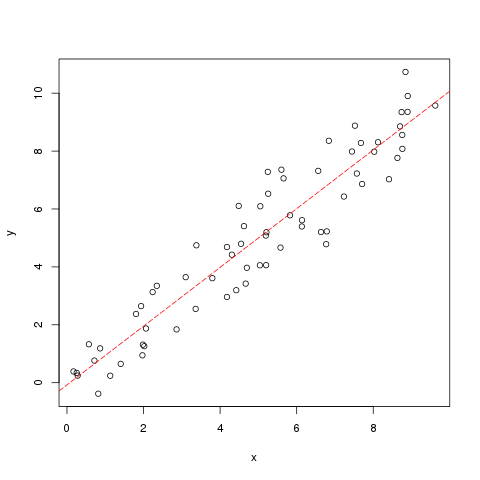
\includegraphics[scale=0.45]{a_regression/ordinary_least_squares_regression_result.png}
\caption{Plot 2D training dataset with the line of best fit.}
\label{plot:ordinary_least_squares_regression_result}
\end{figure}

% other packages ?


% References: Deeper understanding
% The references element description includes a listing of both primary sources of information about the technique as well as useful introductory sources for novices to gain a deeper understanding of the theory and application of the technique. The description consists of hand-selected reference material including books, peer reviewed conference papers, journal articles, and potentially websites. A bullet-pointed structure is suggested.
\subsection{References}
% What are the primary sources for a technique?
% What are the suggested reference sources for learning more about a technique?

% primary sources
\subsubsection{Primary Sources}
% least squares
The method for Least Squares may be traced back to Gauss who claims to have devised the method in and later published it in 1809 \cite{Gauss1809, Gauss1823} (Latin). Legendre independently developed and published the Least Squares method in 1805 \cite{Legendre1805} (Appendix, French).
% ordinary least squares specifically

% more info
\subsubsection{More Information}
% text books
Least Squares Regression is covered in any good text of statistics, data analysis or econometrics. Some popular introductory texts to least squares regression include Montgomery et~al.\ \cite{Montgomery2001} (Chapter 2), and Tamhane and Dunlop \cite{Tamhane2000} (Chapter 10).
% in R
Faraway provides a free book that includes a practical introduction into Least Squares Regression with examples in R \cite{Faraway2002} (updated version published \cite{Faraway2004}).


% END
\putbib\end{bibunit}
\newpage\begin{bibunit}% The Clever Algorithms Project: http://www.CleverAlgorithms.com
% (c) Copyright 2011 Jason Brownlee. Some Rights Reserved. 
% This work is licensed under a Creative Commons Attribution-Noncommercial-Share Alike 2.5 Australia License.

% Name
% The algorithm name defines the canonical name used to refer to the technique, in addition to common aliases, abbreviations, and acronyms. The name is used in terms of the heading and sub-headings of an algorithm description.
\section{Logistic Regression} 
\label{sec:logistic}
\index{Logistic Regression}
\index{logit}

% other names
% What is the canonical name and common aliases for a technique?
% What are the common abbreviations and acronyms for a technique?
\emph{Logistic Regression, Logit, Logit Model, Logistic Model, Binomial Logistic Regression, Binary Logistic Regression}

% Taxonomy: Lineage and locality
\subsection{Taxonomy}
% To what fields of study does a technique belong?
% What are the closely related approaches to a technique?
Logistic Regression is a regression method from the field of statistics, although us better understood as a classification method.
The most common form is Binomial Logistic Regression where the dependent variable is binary.
Logistic Regression may be considered a special case of Generalized Linear Regression.
Logistic Regression has many extensions including Ordered Logistic Regression that can handle ordinal dependent variables, and Multinomial Logistic Regression that can handle nominal (categorical) dependent variables.

What is Weighted Logistic Regression?
What is Stepwise Logistic Regression?
Where does Regularized Logistic Regression fit in?

% Strategy: Problem solving plan
% The strategy is an abstract description of the computational model. The strategy describes the information processing actions a technique shall take in order to achieve an objective. The strategy provides a logical separation between a computational realization (procedure) and a analogous system (metaphor). A given problem solving strategy may be realized as one of a number specific algorithms or problem solving systems. The strategy description is textual using information processing and algorithmic terminology.
\subsection{Strategy}
% What is the information processing objective of a technique?
Logistic Regression fits data to a logistic (sigmoidal) function and makes predictions of the probability of occurrence of an event. 
% What is a techniques plan of action?
A logistic function is used because it can take any values (positive or negative) and produce a value between 0 and 1. The logistic function is influenced by a logit function which take a variable derived from a sum of the weighted attributes. The logit function is the natural logarithm of the odds of the dependent variable equalling one.

The sign of a regression coefficient may be interpreted as the increase or decrease of an attribute to the resulting probability, and the magnitude represents the influence of the attribute.
The regression coefficients (weights) are fit by minimizing the maximum likelihood loss function. The problem as a system of linear equations use the Conjugate Gradient Method to solve the coefficients. Much research into the method is focused on more efficient algorithms for fitting the model.


% help me use this technique
\subsection{Overview}

% what it is good at
\subsubsection{Features}

\begin{itemize}
	\item Generally fast to create and results in an explainable model.
	\item Generally not parametrized, so there are no parameters to configure.
	\item Produces values always between zero and one. 
	\item Does not assume a linear relationship between the independent variables and the dependent variable. 
	\item Does not require normally distributed variables.
	\item The result is a probability of the occurrence of an event that may be interpreted as such and/or in turn be discretized to a binary classification prediction.
	\item More data can result in a better fit of the model.
	\item Training data with a minimum of 10 events per independent variable is recommended \cite{Peduzzi1996}.
	\item Features should be selected prior to fitting.
	\item Provides statistical test significance on a fitted model including: Wald Z-statistic, Likelihood-Ratio Test, and the Hosmer-Lemshow Goodness of Fit Test.
\end{itemize}

% what it is not good at
\subsubsection{Limitations}

\begin{itemize}
	\item The dependent variable must be binary (otherwise one must use another form of the method).
	\item The use of a logistic function means that input attributes can take any value, the bounds do not need to be known prior to building the model.
	\item It can only handle real-valued dependent variables.
	\item Dependent on the size of the sample used to prepare the model, smaller samples ($<1000$ or $<500$) can result in a model that overfits the training data.
	\item Solving the coefficients for large models can be very computationally expensive and remains an open area for research.
	\item Missing values must be handled explicitly or those records removed.
	\item Requires that the independent variable be related to the logit by a linear relationship.
\end{itemize}


% sample script in R
\subsection{Code Listing}
Listing~\ref{glm_logistic} provides a code listing of Logistic Regression in R using the \texttt{glm} (generalized linear model) function of the \texttt{stats} core package. 
% problem
The test problem is a contrived one dimensional problem where given a health statistic ($h$) determine whether a patient will survive or not $s\in\{0,1\}$.
The \texttt{gml} is distributed in core R and provides a number of functions besides the logistic function. By default, the method uses the Iteratively Re-weighted Least Squares (IWLS) method to fit.

% TODO make 2D problem and show the decision boundary + data points
% show stats?
% show convergence of gradient descent?

\lstinputlisting[firstline=7,language=r,caption={Example of Logistic Regression in R using the \texttt{glm} function of the \texttt{stats} core package.}, label=stats_logistic]{../src/algorithms/regression/stats_logistic_regression.R}

% References: Deeper understanding
% The references element description includes a listing of both primary sources of information about the technique as well as useful introductory sources for novices to gain a deeper understanding of the theory and application of the technique. The description consists of hand-selected reference material including books, peer reviewed conference papers, journal articles, and potentially websites. A bullet-pointed structure is suggested.
\subsection{References}
% What are the primary sources for a technique?
% What are the suggested reference sources for learning more about a technique?

% primary sources
\subsubsection{Primary Sources}

What are some primary sources for this method?

% more info
\subsubsection{More Information}
%Komarek and Moore provide promote the use of the method in modern data mining, suggesting modifications to the fit procedure to decrease computational complexity \cite{Komarek2005}.

There are many excellent books dedicated to Logistic Regression, some examples include 
``Logistic Regression: A Primer'' by Pampel that provides a practical introduction to the method \cite{Pampel2000}, ``Applied logistic regression'' by Hosmer and Lemeshow that provides a wealth of references \cite{Hosmer2000}, and ``Logistic Regression: A Self-Learning Text'' by Kleinbaum, Klein, and Pryor that is also an excellent self-paced introductory text \cite{Kleinbaum2010}.


% END\putbib\end{bibunit}
\newpage\begin{bibunit}% The Clever Algorithms Project: http://www.CleverAlgorithms.com
% (c) Copyright 2013 Jason Brownlee. Some Rights Reserved. 
% This work is licensed under a Creative Commons Attribution-Noncommercial-Share Alike 2.5 Australia License.


% Name
% The algorithm name defines the canonical name used to refer to the technique, in addition to common aliases, abbreviations, and acronyms. The name is used in terms of the heading and sub-headings of an algorithm description.
\section{Ridge Regression} 
\label{sec:ridge}
\index{Ridge Regression}
\index{Tikhonov Regularization}
\index{Tikhonov-Miller Method}
\index{Phillips-Twomey Method}
\index{Constrained Linear Inversion}
\index{Linear Regularization}
\index{Penalized $L_2$ Regression}
\index{$L_2$-norm Penalty}

% other names
% What is the canonical name and common aliases for a technique?
% What are the common abbreviations and acronyms for a technique?
\emph{Ridge Regression, Tikhonov Regularization, Tikhonov-Miller Method, Phillips-Twomey Method, Constrained Linear Inversion, Linear Regularization, Penalized $L_2$ Regression}

% Taxonomy: Lineage and locality
% The algorithm taxonomy defines where a techniques fits into the field, both the specific subfields of Computational Intelligence and Biologically Inspired Computation as well as the broader field of Artificial Intelligence. The taxonomy also provides a context for determining the relation- ships between algorithms. The taxonomy may be described in terms of a series of relationship statements or pictorially as a venn diagram or a graph with hierarchical structure.
\subsection{Taxonomy}
% To what fields of study does a technique belong?
Ridge Regression is a Regularization method for Multiple Linear Regression models.
% What are the closely related approaches to a technique?
Ridge Regression is related to other Regularized Regression models such as the LASSO and Elastic Net.
The general method of penalizing a model based on the sum of squared parameters is related to Weight Decay in the training of Artificial Neural Networks.

% Strategy: Problem solving plan
% The strategy is an abstract description of the computational model. The strategy describes the information processing actions a technique shall take in order to achieve an objective. The strategy provides a logical separation between a computational realization (procedure) and a analogous system (metaphor). A given problem solving strategy may be realized as one of a number specific algorithms or problem solving systems. The strategy description is textual using information processing and algorithmic terminology.
\subsection{Strategy}
% What is the information processing objective of a technique?
The information processing objective of Ridge Regression is to reduce or shrink the magnitude of the coefficients in a regression model.
% What is a techniques plan of action?
This is achieved by penalizing models based on the sum of the squared coefficients called an $L_2$ penalty or the $L_2$ norm. This term is added to the regression equation during the preparation of the model and is weighted by a complexity parameter ($\lambda$) that controls the amount of shrinkage of the coefficients. 
The effect is that coefficients of a regression model are shrunk towards zero during the training of the model. The intercept is not penalized.

% Heuristics: Usage guidelines
% The heuristics element describe the commonsense, best practice, and demonstrated rules for applying and configuring a parameterized algorithm. The heuristics relate to the technical details of the techniques procedure and data structures for general classes of application (neither specific implementations not specific problem instances). The heuristics are described textually, such as a series of guidelines in a bullet-point structure.
\subsection{Heuristics}
% What are the suggested configurations for a technique?
% What are the guidelines for the application of a technique to a problem instance?

\begin{itemize}
	\item It commonly results in a model with a better bias-variance trade-off than Ordinary Least Squares.
	\item The ridge constant $\lambda$ is typically selected in the range $[0,1]$, where $\lambda=0$ corresponds to an Ordinary Least Squares regression.
	\item Unlike other selection methods, Ridge Regression does not drop coefficients, all model parameters are maintained at the end of the process providing shrinkage but not selection of parameters.
	\item Inputs are commonly standardized before training the model as models are not equivalent under scaling.
	\item Cross-validation is commonly used to assess the model and model selection or stopping criteria.
	\item It is suited for problems where there are more predictors $p$ than there are observations $n$, $p>n$ problems.
\end{itemize}

% sample script in R
\subsection{Code Listing}
% listing
Listing~\ref{mass_ridge_regression} provides a code listing of the Ridge Regression method in R.
% algorithm and package
The example uses the \texttt{lm.ridge()} function in the \texttt{MASS} core package which is responsible for fitting linear models using Ridge Regression. The example trials a sequence of lambda values then uses the model with the best lambda value for prediction. Figure~\ref{plot:ridge_regression_result} provides a plot of the final coefficient values of each model for the given lambda values. For more information on this library type: \texttt{library(help="MASS")}, and for more information on the function type: \texttt{?lm.ridge}.

% problem
The test problem is a four-dimensional dataset of 100 samples, where \texttt{x3} and \texttt{y} are dependent on \texttt{x1} and \texttt{x1} and \texttt{x2} are independent variables. The problem is ill defined as \texttt{y} given \texttt{x1, x2, x3}. The model is expected to reduce the contribution of \texttt{x2} and \texttt{x3} toward zero leaving \texttt{y} given \texttt{x1}.

\lstinputlisting[firstline=7,language=r,caption={Example of Ridge Regression in R using the \texttt{lm.ridge()} function in the \texttt{MASS} package.}, label=mass_ridge_regression]{../src/algorithms/regularization/mass_ridge_regression.R}

\begin{figure}[htp]
\centering
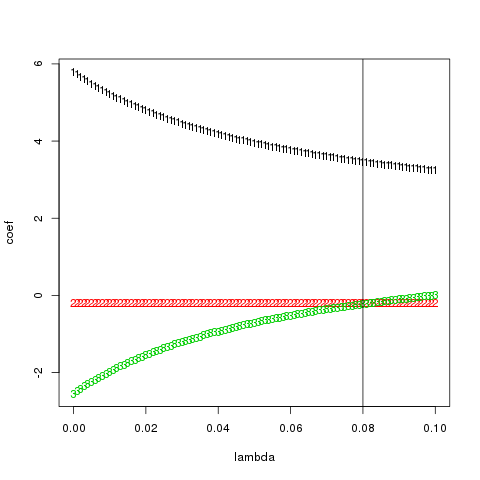
\includegraphics[scale=0.70]{book/a_regularization/ridge_regression_result.png}
\caption{Plot of the final coefficient values of each model for the given lambda values. The numbers reflect the \texttt{x} variables 1, 2 and 3. The line shows a selected lambda value.}
\label{plot:ridge_regression_result}
\end{figure}

% other packages ?
Other packages that provide an implementation of Ridge Regression include \texttt{parcor}.
% penalized package

% References: Deeper understanding
% The references element description includes a listing of both primary sources of information about the technique as well as useful introductory sources for novices to gain a deeper understanding of the theory and application of the technique. The description consists of hand-selected reference material including books, peer reviewed conference papers, journal articles, and potentially websites. A bullet-pointed structure is suggested.
\subsection{References}
% What are the primary sources for a technique?
% What are the suggested reference sources for learning more about a technique?

% primary sources
\subsubsection{Primary Sources}
% seminal
The method was originally described by Tikhonov \cite{Tikhonov1943, Tikhonov1963} (Russian), who later published a full account of the method as a book \cite{Tikhonov1977}.
% others
Phillips independently described the method \cite{Phillips1962}. Hoerl was first to use the term `Ridge Regression' which was adopted in the field of Statistics for $p>n$ problems \cite{Hoerl1962, Hoerl1970, Hoerl1970a}.

% more info
\subsubsection{More Information}
Hastie et~al.\ provide a gentle introduction to the method from the perspective of linear regression (\cite{Hastie2009}, page 61).
% applied
Press et~al.\ provide an introduction to Ridge Regression with examples in the C programming language \cite{Press2007} (Chapter 19).
Faraway provides an introduction to Ridge Regression with examples in R \cite{Faraway2002}.

% END
\putbib\end{bibunit}
\newpage\begin{bibunit}% The Clever Algorithms Project: http://www.CleverAlgorithms.com
% (c) Copyright 2011 Jason Brownlee. Some Rights Reserved. 
% This work is licensed under a Creative Commons Attribution-Noncommercial-Share Alike 2.5 Australia License.

% Name
% The algorithm name defines the canonical name used to refer to the technique, in addition to common aliases, abbreviations, and acronyms. The name is used in terms of the heading and sub-headings of an algorithm description.
\section{Stepwise Linear Regression} 
\label{sec:stepwise}
\index{Stepwise Linear Regression}

% other names
% What is the canonical name and common aliases for a technique?
% What are the common abbreviations and acronyms for a technique?
\emph{Stepwise Linear Regression, Stepwise Selection}

% Taxonomy: Lineage and locality
% The algorithm taxonomy defines where a techniques fits into the field, both the specific subfields of Computational Intelligence and Biologically Inspired Computation as well as the broader field of Artificial Intelligence. The taxonomy also provides a context for determining the relation- ships between algorithms. The taxonomy may be described in terms of a series of relationship statements or pictorially as a venn diagram or a graph with hierarchical structure.
\subsection{Taxonomy}
% To what fields of study does a technique belong?
% What are the closely related approaches to a technique?
Stepwise Regression is a model selection method for selecting a regression model. It is typically applied to Linear Regression and Generalized Linear Regression Models.

% Strategy: Problem solving plan
% The strategy is an abstract description of the computational model. The strategy describes the information processing actions a technique shall take in order to achieve an objective. The strategy provides a logical separation between a computational realization (procedure) and a analogous system (metaphor). A given problem solving strategy may be realized as one of a number specific algorithms or problem solving systems. The strategy description is textual using information processing and algorithmic terminology.
\subsection{Strategy}
% What is the information processing objective of a technique?
% What is a techniques plan of action?

used for feature selection
greedy algorithm - adds the best feature or removes the worst feature each iteration
have to decide when to stop the algorithm - stopping condition - typically done by cross validation
some criteria can be optimized

see \url{http://www.stata.com/support/faqs/stat/stepwise.html}
good example \url{http://cran.r-project.org/doc/contrib/Faraway-PRA.pdf}

% help me use this technique
\subsection{Overview}

% what it is good at
\subsubsection{Features}

\begin{itemize}
	\item Simple method for feature selection.
	\item One of a variety of selection criteria can be used, common examples include the Akaike Information Criterion (AIC), and the Bayes Information Criterion (BIC).
\end{itemize}

% what it is not good at
\subsubsection{Limitations}

\begin{itemize}
	\item Stepwise models are a deprecated method as they have a high chance of selecting the wrong attributes and being optimistic of the model they prepare.
\end{itemize}



% sample script in R
\subsection{Code Listing}
% listing
Listing~\ref{stats_stepwise_linear_regression} provides a code listing of Stepwise Linear Regression method in R to find the relevant features and the line of best fit for those features.
% algorithm and package
The example uses the {lm()} function and the and \texttt{step()} in the \texttt{stats} core package which are responsible for fitting linear models and performing stepwise selection respectively. The \texttt{step()} function uses a Akaike Information Criterion as the model evaluation criteria.

% problem
The test problem is a four-dimensional dataset of 50 samples, where the x-values are drawn from a uniformly random distribution $x \in [0,10]$ and \texttt{y} values are dependent on the \texttt{x} value plus a value drawn from a normally random distribution with a mean of 0 and a standard deviation of 1. The features \texttt{a} and \texttt{b} are random independent variables that have no relevant interaction x and y. In this example, \texttt{y} is considered the dependent variable and x the single relevant independent. The stepwise method is expected to discount \texttt{a} and \texttt{b} and select a linear model for \texttt{y} given \texttt{x}.

% classification example?

\lstinputlisting[firstline=7,language=r,caption={Example of Stepwise Linear Regression in R using the \texttt{lm()} and \texttt{step()} functions in the \texttt{stats} core package.}, label=stats_stepwise_linear_regression]{../src/algorithms/regression/stats_stepwise_linear_regression.R}

% other packages
Other packages that provide stepwise selection include the \texttt{stepAIC} function of the \texttt{MASS} package. The \texttt{leaps} package does not provide stepwise selection, although does provides a related selection method called Regression Subset Selection that uses a branch and bound search.


% References: Deeper understanding
% The references element description includes a listing of both primary sources of information about the technique as well as useful introductory sources for novices to gain a deeper understanding of the theory and application of the technique. The description consists of hand-selected reference material including books, peer reviewed conference papers, journal articles, and potentially websites. A bullet-pointed structure is suggested.
\subsection{References}
% What are the primary sources for a technique?
% What are the suggested reference sources for learning more about a technique?

% primary sources
\subsubsection{Primary Sources}


Great early overview of the approaches (forward and backward selection) \cite{Hocking1976}.

% more info
\subsubsection{More Information}

arguments against it in modern analysis
Overview of why using stepwise regression is a bad idea \cite{Whittingham2006}.
\cite{Mundry2009}





% END
\putbib\end{bibunit}
\newpage\begin{bibunit}% The Clever Algorithms Project: http://www.CleverAlgorithms.com
% (c) Copyright 2011 Jason Brownlee. Some Rights Reserved. 
% This work is licensed under a Creative Commons Attribution-Noncommercial-Share Alike 2.5 Australia License.

% Name
% The algorithm name defines the canonical name used to refer to the technique, in addition to common aliases, abbreviations, and acronyms. The name is used in terms of the heading and sub-headings of an algorithm description.
\section{Multivariate Adaptive Regression Splines} 
\label{sec:mars}
\index{Multivariate Adaptive Regression Splines}
\index{MARS}
\index{MARSplines}
\index{Adaptive Regression Splines}

% other names
% What is the canonical name and common aliases for a technique?
% What are the common abbreviations and acronyms for a technique?
\emph{Multivariate Adaptive Regression Splines, MARS, MARSplines, Adaptive Regression Splines.}

% Taxonomy: Lineage and locality
% The algorithm taxonomy defines where a techniques fits into the field, both the specific subfields of Computational Intelligence and Biologically Inspired Computation as well as the broader field of Artificial Intelligence. The taxonomy also provides a context for determining the relation- ships between algorithms. The taxonomy may be described in terms of a series of relationship statements or pictorially as a venn diagram or a graph with hierarchical structure.
\subsection{Taxonomy}
% To what fields of study does a technique belong?
Multivariate Adaptive Regression Splines is a Multivariate Non-Parametric Regression method.
% What are the closely related approaches to a technique?
It is related to other Non-Parametric Regression methods such as Kernel Regression, Non-Parametric Multiplicative Regression, Additive Modelling and Regression Trees. The procedure to prepare the model is related to Regressive Partitioning for decision trees (CART). The use of forward and backward phases in regression shows some similarity to Stepwise Regression.
% extensions
Fast MARS in an extension of the canonical MARS method that suggests an optimization of the forward procedure when building the model.
% PolyMars?

% Strategy: Problem solving plan
% The strategy is an abstract description of the computational model. The strategy describes the information processing actions a technique shall take in order to achieve an objective. The strategy provides a logical separation between a computational realization (procedure) and a analogous system (metaphor). A given problem solving strategy may be realized as one of a number specific algorithms or problem solving systems. The strategy description is textual using information processing and algorithmic terminology.
\subsection{Strategy}
% What is the information processing objective of a technique?
The information processing objective of the technique is to find an equation that best describes the relationships between independent and a dependent variable.
% What is the model?
This is achieved by preparing a model that is the weighted sum of basis functions. A basis function can be as simple as a constant, or as complex as one or the product of multiple sub-functions that add non-linearities called hinge functions. Hinge functions take the form of $max(0, x-c)$ where $0$ is the minimum value for the function, $x$ is the variable, and $c$ is a constant (that provides a kink or sharp turn in one-dimension) called the knot. The number of basis functions as well as the parameters for each are determined determined automatically through an iterative process based on the data.

% what is the algorithm to arrive at the model?
MARS is motivated as a process to create a continuous model using a procedure like that used in recursive partitioning (CART). Like recursive partitioning, the method has a forward procedure to add terms and a backward procedure to prune terms from the model.
% forward
The forward procedure is a greedy algorithm that seeks to minimizes the sum of squared residual errors (SSR). It starts with the intercept and adds basis function terms to the model until a maximum number of terms have been added or no further improvements in SSR are possible. Terms are added and configured to give the greatest reduction in SSR.

% backward
The intent of the forward procedure is overfit the training data. The backward step is intended to add generality to the mode by pruning terms one-at-a-time selecting each term to remove based on the improvement in a generalized cross-validation score. The backward pass typically prunes one side of each pair of terms.
% cross validation score
The generalized cross-validation score is a performance measure that takes the complexity of the model and size of the training dataset as well as the SSR into account. The score seeks to minimize for model flexibility.

% Heuristics: Usage guidelines
% The heuristics element describe the commonsense, best practice, and demonstrated rules for applying and configuring a parameterized algorithm. The heuristics relate to the technical details of the techniques procedure and data structures for general classes of application (neither specific implementations not specific problem instances). The heuristics are described textually, such as a series of guidelines in a bullet-point structure.
\subsection{Heuristics}
% What are the suggested configurations for a technique?
% What are the guidelines for the application of a technique to a problem instance?

\begin{itemize}
	\item Friedman originally proposed it a suitable technique for sample sizes $50 \leq N \leq 1000$ and dimensions $3 \leq n \leq 20$.
	\item The algorithm requires the specification of the maximum number of terms to add in the forward pass. % recommended values?
	\item A penalty term (\texttt{d}) is used on the generalized cross-validation score which is commonly set to a small integer value ($d<4$, typically 2 or 3).
	\item Constraints can be imposed on the addition of terms in the first pass, such as limitations on the number of interactions permitted between basis functions. Low numbers of interactions are common (such as 1 or 2).
	\item It may be more suitable to real valued variables than recursive partitioning given the continuous nature of the hinge basis functions.
	\item Like partitioning, data preparation may not required as the hinge functions can account for outliers.
	\item The training times for MARS are relatively fast although it is a generally slower process than Recursive Partitioning on the same training dataset.
\end{itemize}

% sample script in R
\subsection{Code Listing}
% listing
Listing~\ref{earth_multivariate_adaptive_regression_splines} provides a code listing Multivariate Adaptive Regression Splines method in R to find a line of best fit for a two-dimensional data set.
% algorithm and package
The example uses the {earth()} function in the \texttt{earth} package that uses a generalized linear model as the underling method.
% problem
The test problem is a two-dimensional dataset of 50 samples, where the x-values are drawn from a uniformly random distribution $x \in [0,10]$ and y values are the x value plus a value drawn from a normally random distribution with a mean of 0 and a standard deviation of 1.

% code listing
\lstinputlisting[firstline=7,language=r,caption={Example of Multivariate Adaptive Regression Splines in R using the \texttt{earth} function of the \texttt{earth} package.}, label=earth_multivariate_adaptive_regression_splines]{../src/algorithms/regression/earth_multivariate_adaptive_regression_splines.R}

% other code examples
For more information on the \texttt{earth} package and function type \texttt{?earth}. Foulkes provides an example of using the \texttt{earth} package for genetic analysis \cite{Foulkes2009}. Mills provides an example using the \texttt{earth} package with sample output and plots of the model \cite{Mills2010}. Torgo also provides a small example if using the \texttt(earth) package \cite{Torgo2009}. 
% other package
Some other packages that provide an implementation of MARS include the \texttt{mda} package and the \texttt{polymars} package.


% References: Deeper understanding
% The references element description includes a listing of both primary sources of information about the technique as well as useful introductory sources for novices to gain a deeper understanding of the theory and application of the technique. The description consists of hand-selected reference material including books, peer reviewed conference papers, journal articles, and potentially websites. A bullet-pointed structure is suggested.
\subsection{References}
% What are the primary sources for a technique?
% What are the suggested reference sources for learning more about a technique?

% primary sources
\subsubsection{Primary Sources}
% seminal
MARS was proposed by Friedman in a paper that walks through the method in great detail and provides a number of case study datasets \cite{Friedman1991}.
% variable types
The approach was extended by Friedman to support both ordinal and categorical variables and missing values for this variable type \cite{Friedman1991a, Friedman1993a}.

% more info
\subsubsection{More Information}
% neural nets
The capability of representing non-linear relationships in the model using a number of basis functions likens the approach to artificial neural networks Friedman described the method in the context of neural networks, referring to it as `Adaptive Spline Networks' \cite{Friedman1991b, Friedman1991c}.
% Fast MARS
Friedman also suggested an improvement to optimize the forward pass procedure of the algorithm for large datasets called Fast MARS \cite{Friedman1993}.

% reviews
Friedman and Roosen provide an early introduction to the method with sample output from the FORTRAN program and clinical case studies \cite{Friedman1995}.
% R
Faraway provides a modern summary of the method and provides an example of using MARS using R \cite{Faraway2006} (page 271).


% END
\putbib\end{bibunit}
\newpage\begin{bibunit}% The Clever Algorithms Project: http://www.CleverAlgorithms.com
% (c) Copyright 2011 Jason Brownlee. Some Rights Reserved. 
% This work is licensed under a Creative Commons Attribution-Noncommercial-Share Alike 2.5 Australia License.

% Name
% The algorithm name defines the canonical name used to refer to the technique, in addition to common aliases, abbreviations, and acronyms. The name is used in terms of the heading and sub-headings of an algorithm description.
\section{Linear Discriminant Analysis} 
\label{sec:lda}
\index{Linear Discriminant Analysis}
\index{Linear Discriminant Function}
\index{Discriminant Analysis}
\index{LDA}

% other names
% What is the canonical name and common aliases for a technique?
% What are the common abbreviations and acronyms for a technique?
\emph{Linear Discriminant Analysis, Discriminant Analysis, Discriminant Function Analysis, Linear Discriminant Function, LDA.}

% Taxonomy: Lineage and locality
% The algorithm taxonomy defines where a techniques fits into the field, both the specific subfields of Computational Intelligence and Biologically Inspired Computation as well as the broader field of Artificial Intelligence. The taxonomy also provides a context for determining the relation- ships between algorithms. The taxonomy may be described in terms of a series of relationship statements or pictorially as a venn diagram or a graph with hierarchical structure.
\subsection{Taxonomy}
% To what fields of study does a technique belong?
% What are the closely related approaches to a technique?
Linear Discriminant Analysis is a classification method.

Used for classification and for dimensionality reduction.

What is Fisher Linear Discriminant Analysis?

How is it related to Quadratic Discriminant Analysis?
Factor Analysis?
PCA

Related to linear regression which provides a linear model for a numeric rather than categorical.


% Strategy: Problem solving plan
% The strategy is an abstract description of the computational model. The strategy describes the information processing actions a technique shall take in order to achieve an objective. The strategy provides a logical separation between a computational realization (procedure) and a analogous system (metaphor). A given problem solving strategy may be realized as one of a number specific algorithms or problem solving systems. The strategy description is textual using information processing and algorithmic terminology.
\subsection{Strategy}
% What is the information processing objective of a technique?
% What is a techniques plan of action?

used for classification and dimensionality reduction
kind of like regression
linear model for a nominal (categorical) dependent variable.


% help me use this technique
\subsection{Overview}

% what it is good at
\subsubsection{Features}

\begin{itemize}
	\item Used for prediction of a nominal (categorical) dependent variable, cannot be used for regression.
\end{itemize}

% what it is not good at
\subsubsection{Limitations}

\begin{itemize}
	\item 
\end{itemize}


% sample script in R
\subsection{Code Listing}

MASS package has LDA

see \url{http://www.statmethods.net/advstats/discriminant.html}

% References: Deeper understanding
% The references element description includes a listing of both primary sources of information about the technique as well as useful introductory sources for novices to gain a deeper understanding of the theory and application of the technique. The description consists of hand-selected reference material including books, peer reviewed conference papers, journal articles, and potentially websites. A bullet-pointed structure is suggested.
\subsection{References}
% What are the primary sources for a technique?
% What are the suggested reference sources for learning more about a technique?

% primary sources
\subsubsection{Primary Sources}



% more info
\subsubsection{More Information}





% END
\putbib\end{bibunit}
\newpage\begin{bibunit}% The Clever Algorithms Project: http://www.CleverAlgorithms.com
% (c) Copyright 2011 Jason Brownlee. Some Rights Reserved. 
% This work is licensed under a Creative Commons Attribution-Noncommercial-Share Alike 2.5 Australia License.

% Name
% The algorithm name defines the canonical name used to refer to the technique, in addition to common aliases, abbreviations, and acronyms. The name is used in terms of the heading and sub-headings of an algorithm description.
\section{Locally Estimated Scatterplot Smoothing} 
\label{sec:loess}
\index{Locally Weighted Regression}
\index{LOESS}
\index{LOWESS}
\index{Locally Estimated Scatterplot Smoothing}
\index{Locally Weighted Scatterplot Smoothing}

% other names
% What is the canonical name and common aliases for a technique?
% What are the common abbreviations and acronyms for a technique?
\emph{Locally Weighted Regression, LWR, Locally Estimated Scatterplot Smoothing, LOESS.}

% Taxonomy: Lineage and locality
% The algorithm taxonomy defines where a techniques fits into the field, both the specific subfields of Computational Intelligence and Biologically Inspired Computation as well as the broader field of Artificial Intelligence. The taxonomy also provides a context for determining the relation- ships between algorithms. The taxonomy may be described in terms of a series of relationship statements or pictorially as a venn diagram or a graph with hierarchical structure.
\subsection{Taxonomy}
% To what fields of study does a technique belong?
Locally Weighted Regression known as Locally Estimated Scatterplot Smoothing (LOESS) is a type of Local Regression and belong to the general class of Non-Parametric Regression methods. It also belongs to the framework of Generalized Additive Models (GAMs).
% What are the closely related approaches to a technique?
LOESS is an extension to its precursor method Locally Weighted Scatterplot Smoothing (LOWESS).
It is related to other Non-Parametric Regression methods such as Multivariate Adaptive Regression Splines (MARS), Non-Parametric Multiplicative Regression, Additive Regression Model and Regression Trees. 

% Strategy: Problem solving plan
% The strategy is an abstract description of the computational model. The strategy describes the information processing actions a technique shall take in order to achieve an objective. The strategy provides a logical separation between a computational realization (procedure) and a analogous system (metaphor). A given problem solving strategy may be realized as one of a number specific algorithms or problem solving systems. The strategy description is textual using information processing and algorithmic terminology.
\subsection{Strategy}
% What is the information processing objective of a technique?
The information processing objective of the technique is to find an equation that best describes the relationships between independent and a dependent variable.
% What is a techniques plan of action?


% Heuristics: Usage guidelines
% The heuristics element describe the commonsense, best practice, and demonstrated rules for applying and configuring a parameterized algorithm. The heuristics relate to the technical details of the techniques procedure and data structures for general classes of application (neither specific implementations not specific problem instances). The heuristics are described textually, such as a series of guidelines in a bullet-point structure.
\subsection{Heuristics}
% What are the suggested configurations for a technique?
% What are the guidelines for the application of a technique to a problem instance?

\begin{itemize}
	\item The method is well suited to problems of time series prediction and two-dimensional data exploration (by projecting the line on a scatter plot of the data).
\end{itemize}


% sample script in R
\subsection{Code Listing}


% other packages
The \texttt{lowess} package provides an implementation of LOWESS Scatter Plot Smoothing, a pre-cursor to LOESS regression.

lowess
loess package/function
gam package/function

% References: Deeper understanding
% The references element description includes a listing of both primary sources of information about the technique as well as useful introductory sources for novices to gain a deeper understanding of the theory and application of the technique. The description consists of hand-selected reference material including books, peer reviewed conference papers, journal articles, and potentially websites. A bullet-pointed structure is suggested.
\subsection{References}
% What are the primary sources for a technique?
% What are the suggested reference sources for learning more about a technique?

% primary sources
\subsubsection{Primary Sources}
% precursor
Cleveland described a form of univariate local regression called Locally Weighted Scatterplot Smoothing (LOWESS) which also included a robust version of the method \cite{Cleveland1978, Cleveland1979}. 
This method was extended to the multivariate case by Devlin in an unpublished technical report \cite{Devlin1986}.
% seminal
Locally Estimated Scatterplot Smoothing (LOESS) or Multivariate Locally Weighted Regression is credited to Cleveland and Devlin \cite{Cleveland1988}.

% more info
\subsubsection{More Information}
% precursor
Cleveland presented a FORTRAN routine for LOWESS for data exploration \cite{Cleveland1981}.
% follow-ups
LOESS was further described by Cleveland et~al.\ \cite{Cleveland1988a}.
% implementation
LOESS was further developed by Cleveland and Grosse \cite{Cleveland1991} and later well described in terms of an implementation in S (Rs pre-cursor) \cite{Cleveland1992}.
% modern
Cleveland and Loader provide a more recent salient description of local regression including the history of the general method and examples \cite{Cleveland1996}.

% END
\putbib\end{bibunit}


		% The Clever Algorithms Project: http://www.CleverAlgorithms.com
% (c) Copyright 2010 Jason Brownlee. Some Rights Reserved. 
% This work is licensed under a Creative Commons Attribution-Noncommercial-Share Alike 2.5 Australia License.

% This is a chapter

\renewcommand{\bibsection}{\subsection{\bibname}}
\begin{bibunit}

\chapter{Decision Trees}
\label{ch:trees}
\index{Decision Trees}
\index{Trees}

\section{Overview}
This chapter describes Decision Trees.


% Strategy: Problem solving plan
% The strategy is an abstract description of the computational model. The strategy describes the information processing actions a technique shall take in order to achieve an objective. The strategy provides a logical separation between a computational realization (procedure) and a analogous system (metaphor). A given problem solving strategy may be realized as one of a number specific algorithms or problem solving systems. The strategy description is textual using information processing and algorithmic terminology.
\subsection{Strategy}
% What is the information processing objective of a technique?
% What is a techniques plan of action?

grow a tree from data

prune a tree using cost-complexity graph, (alpha is a meta parameter that controls the degree of stabilization.)

handle huge data sets - divide conquer 
handle mixed features
ignore redundant variables
small are easy to under stand
large are hard to understand
prediction performance is very poor

use cost complexity pruning


% Heuristics: Usage guidelines
% The heuristics element describe the commonsense, best practice, and demonstrated rules for applying and configuring a parameterized algorithm. The heuristics relate to the technical details of the techniques procedure and data structures for general classes of application (neither specific implementations not specific problem instances). The heuristics are described textually, such as a series of guidelines in a bullet-point structure.
\subsection{Heuristics}
% What are the suggested configurations for a technique?
% What are the guidelines for the application of a technique to a problem instance?

\begin{itemize}
	\item Trees are fast to train (simple growing algorithm).
	\item Trees can handle missing values (treat missing as a value, surrogate splits)
	\item Few tunable parameters
	\item Trees can explain why they make their decisions, the tree model can be understood by subject matter experts.
	\item Trees cannot addres curved decision surfaces at all or very well.
	\item Trees generally have hard or blocky decision surfaces.
	\item Trees generally perform poorly across a range of problems.


	% limitations
	\item Need a lot of data to have a lot of splits
	\item Can run out of data after only a few splits in high-dimensions
	\item Each split reduces the data available for subsequent splits (data fragmentation)
	\item Performs poorly if the target function has many dependent variables 
	\item high variance - small changes in training data result in very different trees
	\item errors / decisions made early propagate through the rest of the tree
	\item pruning is important

\end{itemize}



% References: Deeper understanding
% The references element description includes a listing of both primary sources of information about the technique as well as useful introductory sources for novices to gain a deeper understanding of the theory and application of the technique. The description consists of hand-selected reference material including books, peer reviewed conference papers, journal articles, and potentially websites. A bullet-pointed structure is suggested.
\subsection{References}
% What are the primary sources for a technique?
% What are the suggested reference sources for learning more about a technique?

% primary sources
\subsubsection{Primary Sources}


% more info
\subsubsection{More Information}



\putbib
\end{bibunit}

\newpage\begin{bibunit}% The Clever Algorithms Project: http://www.CleverAlgorithms.com
% (c) Copyright 2011 Jason Brownlee. Some Rights Reserved. 
% This work is licensed under a Creative Commons Attribution-Noncommercial-Share Alike 2.5 Australia License.

% Name
% The algorithm name defines the canonical name used to refer to the technique, in addition to common aliases, abbreviations, and acronyms. The name is used in terms of the heading and sub-headings of an algorithm description.
\section{Recursive Partitioning} 
\label{sec:rpart}
\index{Recursive Partitioning}
\index{Rpart}
\index{Regression Tree}

% other names
% What is the canonical name and common aliases for a technique?
% What are the common abbreviations and acronyms for a technique?
\emph{Recursive Partitioning, Rpart, Regression Tree}

% Taxonomy: Lineage and locality
% The algorithm taxonomy defines where a techniques fits into the field, both the specific subfields of Computational Intelligence and Biologically Inspired Computation as well as the broader field of Artificial Intelligence. The taxonomy also provides a context for determining the relation- ships between algorithms. The taxonomy may be described in terms of a series of relationship statements or pictorially as a venn diagram or a graph with hierarchical structure.
\subsection{Taxonomy}
% To what fields of study does a technique belong?
% What are the closely related approaches to a technique?
Recursive Partitioning is a tree method.


% Strategy: Problem solving plan
% The strategy is an abstract description of the computational model. The strategy describes the information processing actions a technique shall take in order to achieve an objective. The strategy provides a logical separation between a computational realization (procedure) and a analogous system (metaphor). A given problem solving strategy may be realized as one of a number specific algorithms or problem solving systems. The strategy description is textual using information processing and algorithmic terminology.
\subsection{Strategy}
% What is the information processing objective of a technique?
% What is a techniques plan of action?


% help me use this technique
\subsection{Overview}

% what it is good at
\subsubsection{Features}

\begin{itemize}
	\item 
\end{itemize}

% what it is not good at
\subsubsection{Limitations}

\begin{itemize}
	\item 
\end{itemize}


% sample script in R
\subsection{Code Listing}

see the rpart function
see \url{http://i2pi.com/rez/ml_talk/ml_demo.R}


% References: Deeper understanding
% The references element description includes a listing of both primary sources of information about the technique as well as useful introductory sources for novices to gain a deeper understanding of the theory and application of the technique. The description consists of hand-selected reference material including books, peer reviewed conference papers, journal articles, and potentially websites. A bullet-pointed structure is suggested.
\subsection{References}
% What are the primary sources for a technique?
% What are the suggested reference sources for learning more about a technique?

% primary sources
\subsubsection{Primary Sources}


% more info
\subsubsection{More Information}



% END
\putbib\end{bibunit}
\newpage\begin{bibunit}% The Clever Algorithms Project: http://www.CleverAlgorithms.com
% (c) Copyright 2013 Jason Brownlee. Some Rights Reserved. 
% This work is licensed under a Creative Commons Attribution-Noncommercial-Share Alike 2.5 Australia License.


% Name
% The algorithm name defines the canonical name used to refer to the technique, in addition to common aliases, abbreviations, and acronyms. The name is used in terms of the heading and sub-headings of an algorithm description.
\section{Classification And Regression Tree}
\label{sec:cart}
\index{CART}
\index{Classification And Regression Tree}

% other names
% What is the canonical name and common aliases for a technique?
% What are the common abbreviations and acronyms for a technique?
\emph{Classification And Regression Tree, CART.}

% Taxonomy: Lineage and locality
% The algorithm taxonomy defines where a techniques fits into the field, both the specific subfields of Computational Intelligence and Biologically Inspired Computation as well as the broader field of Artificial Intelligence. The taxonomy also provides a context for determining the relation- ships between algorithms. The taxonomy may be described in terms of a series of relationship statements or pictorially as a venn diagram or a graph with hierarchical structure.
\subsection{Taxonomy}
% To what fields of study does a technique belong?
% What are the closely related approaches to a technique?
The Classification And Regression Tree or CART is a Decision Tree algorithm. CART is a registered trademark.

% Strategy: Problem solving plan
% The strategy is an abstract description of the computational model. The strategy describes the information processing actions a technique shall take in order to achieve an objective. The strategy provides a logical separation between a computational realization (procedure) and a analogous system (metaphor). A given problem solving strategy may be realized as one of a number specific algorithms or problem solving systems. The strategy description is textual using information processing and algorithmic terminology.
\subsection{Strategy}
% What is the information processing objective of a technique?
% What is a techniques plan of action?
A textual description of the information processing strategy.



% help me use this technique
\subsection{Overview}

% what it is good at
\subsubsection{Features}

\begin{itemize}
	\item The algorithm is non-parametric.
	\item The algorithms can be used to create classification and regression trees.
\end{itemize}

% what it is not good at
\subsubsection{Limitations}

\begin{itemize}
	\item 
\end{itemize}




% sample script in R
\subsection{Code Listing}
% listing
Listing~\ref{rpart_cart} provides a code listing of the CART method in R to classify examples from a three-dimensional dataset.
% algorithm and package
The example uses the \texttt{rpart()} function (recursive partitioning) in the \texttt{rpart} package \cite{Meyer2011}.
% TODO more about the package and the functions capabilities

% problem
The test problem is a three-dimensional classification problem, where the $x$ and $y$ attributes are numerical and drawn from normal distributions around 0 and 4. A class value of 0 or 1 is assigned to each coordinate such that the two classes can be separated by a straight line. The dataset is split into a training set to make the model comprised of 67\% of the samples, and a test set for assessing the model comprised of 33\% of the samples.

% TODO provide prediction example

% code listing
\lstinputlisting[firstline=7,language=r,caption={Example of CART in R using the \texttt{rpart()} function of the \texttt{rpart} package.}, label=rpart_cart]{../src/algorithms/trees/rpart_cart.R}

% other packages
Other packages provide implementations of the CART method, such as the \texttt{tree} package.


% References: Deeper understanding
% The references element description includes a listing of both primary sources of information about the technique as well as useful introductory sources for novices to gain a deeper understanding of the theory and application of the technique. The description consists of hand-selected reference material including books, peer reviewed conference papers, journal articles, and potentially websites. A bullet-pointed structure is suggested.
\subsection{References}
% What are the primary sources for a technique?
% What are the suggested reference sources for learning more about a technique?

% primary sources
\subsubsection{Primary Sources}

Seminal reference is the book \cite{Breiman1984}.

% more info
\subsubsection{More Information}



% END
\putbib\end{bibunit}
\newpage\begin{bibunit}% The Clever Algorithms Project: http://www.CleverAlgorithms.com
% (c) Copyright 2013 Jason Brownlee. Some Rights Reserved. 
% This work is licensed under a Creative Commons Attribution-Noncommercial-Share Alike 2.5 Australia License.


% Name
% The algorithm name defines the canonical name used to refer to the technique, in addition to common aliases, abbreviations, and acronyms. The name is used in terms of the heading and sub-headings of an algorithm description.
\section{C4.5} 
\label{sec:c4.5}
\index{C4.5}

% other names
% What is the canonical name and common aliases for a technique?
% What are the common abbreviations and acronyms for a technique?
\emph{C4.5.}

% Taxonomy: Lineage and locality
% The algorithm taxonomy defines where a techniques fits into the field, both the specific subfields of Computational Intelligence and Biologically Inspired Computation as well as the broader field of Artificial Intelligence. The taxonomy also provides a context for determining the relation- ships between algorithms. The taxonomy may be described in terms of a series of relationship statements or pictorially as a venn diagram or a graph with hierarchical structure.
\subsection{Taxonomy}
% To what fields of study does a technique belong?
% What are the closely related approaches to a technique?
C4.5 is a Decision Tree algorithm.

% Strategy: Problem solving plan
% The strategy is an abstract description of the computational model. The strategy describes the information processing actions a technique shall take in order to achieve an objective. The strategy provides a logical separation between a computational realization (procedure) and a analogous system (metaphor). A given problem solving strategy may be realized as one of a number specific algorithms or problem solving systems. The strategy description is textual using information processing and algorithmic terminology.
\subsection{Strategy}
% What is the information processing objective of a technique?
% What is a techniques plan of action?
A textual description of the information processing strategy.

% Heuristics: Usage guidelines
% The heuristics element describe the commonsense, best practice, and demonstrated rules for applying and configuring a parameterized algorithm. The heuristics relate to the technical details of the techniques procedure and data structures for general classes of application (neither specific implementations not specific problem instances). The heuristics are described textually, such as a series of guidelines in a bullet-point structure.
\subsection{Heuristics}
% What are the suggested configurations for a technique?
% What are the guidelines for the application of a technique to a problem instance?

\begin{itemize}
	\item todo
\end{itemize}


J4.8 from WEKA provides a version of C4.5


% References: Deeper understanding
% The references element description includes a listing of both primary sources of information about the technique as well as useful introductory sources for novices to gain a deeper understanding of the theory and application of the technique. The description consists of hand-selected reference material including books, peer reviewed conference papers, journal articles, and potentially websites. A bullet-pointed structure is suggested.
\subsection{References}
% What are the primary sources for a technique?
% What are the suggested reference sources for learning more about a technique?

% primary sources
\subsubsection{Primary Sources}

Book \cite{Quinlan1993}.

% more info
\subsubsection{More Information}



% END
\putbib\end{bibunit}

		\include{c_kernels}
		% The Clever Algorithms Project: http://www.CleverAlgorithms.com
% (c) Copyright 2010 Jason Brownlee. Some Rights Reserved. 
% This work is licensed under a Creative Commons Attribution-Noncommercial-Share Alike 2.5 Australia License.

% This is a chapter

\renewcommand{\bibsection}{\subsection{\bibname}}
\begin{bibunit}

\chapter{Ensembles}
\label{ch:ensembles}
\index{Ensembles}

\section{Overview}
This chapter describes Ensembles methods.


% Strategy: Problem solving plan
% The strategy is an abstract description of the computational model. The strategy describes the information processing actions a technique shall take in order to achieve an objective. The strategy provides a logical separation between a computational realization (procedure) and a analogous system (metaphor). A given problem solving strategy may be realized as one of a number specific algorithms or problem solving systems. The strategy description is textual using information processing and algorithmic terminology.
\subsection{Strategy}
% What is the information processing objective of a technique?
% What is a techniques plan of action?


efficient - weak learners are easier to train than finding the best model
difficulty in selecting a model
Weak learner and basis function are synonyms.
There is now theory on why ensembles work (performing a Monte Carlo simulation for an integration problem).
Best results from combining low bias, high-variance learners

strategies
- vary the models (functions)
- vary the data

compmenent of model selection - combines measures of fit in cross validation
ensembles combine fitted values (predictions)


BOOSTING
prepare each tree on a weighted sample
fix the mistakes made before
more clever version of bagging
build tree, assign weights based on mistakes, build next tree, so on
weighted averages of observations when splitting

gradient descent of a loss function... modern understanding - gradient boosting

control the size of the trees - quite small - faster

train beyond perfect train data - test error gets better!
makes the problem harder and harder - but the error does start increasing again

MODERN:
building an expanding basis function - stepwise additive modelling - does it iteratively - forward stage wise learning
like basis pursuit is of the same form - matching pursuit




% Heuristics: Usage guidelines
% The heuristics element describe the commonsense, best practice, and demonstrated rules for applying and configuring a parameterized algorithm. The heuristics relate to the technical details of the techniques procedure and data structures for general classes of application (neither specific implementations not specific problem instances). The heuristics are described textually, such as a series of guidelines in a bullet-point structure.
\subsection{Heuristics}
% What are the suggested configurations for a technique?
% What are the guidelines for the application of a technique to a problem instance?


\begin{itemize}
	\item Many weak learners can out-perform a single strong learner.
	\item The diversity of the ensemble set is important property of success. Don't want all models to tell the same story - want different points of view.
	\item Model must be better than random, models must be independent (data, modeled function, etc).
\end{itemize}


% References: Deeper understanding
% The references element description includes a listing of both primary sources of information about the technique as well as useful introductory sources for novices to gain a deeper understanding of the theory and application of the technique. The description consists of hand-selected reference material including books, peer reviewed conference papers, journal articles, and potentially websites. A bullet-pointed structure is suggested.
\subsection{References}
% What are the primary sources for a technique?
% What are the suggested reference sources for learning more about a technique?

% primary sources
\subsubsection{Primary Sources}



% more info
\subsubsection{More Information}

Early overview that was cited a lot \cite{Dietterich2000}.

\putbib
\end{bibunit}


\newpage\begin{bibunit}% The Clever Algorithms Project: http://www.CleverAlgorithms.com
% (c) Copyright 2011 Jason Brownlee. Some Rights Reserved. 
% This work is licensed under a Creative Commons Attribution-Noncommercial-Share Alike 2.5 Australia License.

% Name
% The algorithm name defines the canonical name used to refer to the technique, in addition to common aliases, abbreviations, and acronyms. The name is used in terms of the heading and sub-headings of an algorithm description.
\section{Bootstrapped Aggregation} 
\label{sec:bagging}
\index{Bagging}
\index{Bootstrapped Aggregation}

% other names
% What is the canonical name and common aliases for a technique?
% What are the common abbreviations and acronyms for a technique?
\emph{Bagging, Bootstrapped Aggregation}

% Taxonomy: Lineage and locality
% The algorithm taxonomy defines where a techniques fits into the field, both the specific subfields of Computational Intelligence and Biologically Inspired Computation as well as the broader field of Artificial Intelligence. The taxonomy also provides a context for determining the relation- ships between algorithms. The taxonomy may be described in terms of a series of relationship statements or pictorially as a venn diagram or a graph with hierarchical structure.
\subsection{Taxonomy}
% To what fields of study does a technique belong?
% What are the closely related approaches to a technique?
Bootstrapped Aggregation (Bagging) is an Ensemble algorithm.
Bagging is a special case of Stagewise Additive Modeling - General Forward Stagewise Additive Modeling


% Strategy: Problem solving plan
% The strategy is an abstract description of the computational model. The strategy describes the information processing actions a technique shall take in order to achieve an objective. The strategy provides a logical separation between a computational realization (procedure) and a analogous system (metaphor). A given problem solving strategy may be realized as one of a number specific algorithms or problem solving systems. The strategy description is textual using information processing and algorithmic terminology.
\subsection{Strategy}
% What is the information processing objective of a technique?
% What is a techniques plan of action

a variance reduction technique
 each partition is an iid

partition data into random subsets, with replacement - called bootstrap replicates
train a model on each partition
average the results

not suited to all models - not good for svm
svm variance is not high

% help me use this technique
\subsection{Overview}

% what it is good at
\subsubsection{Features}

\begin{itemize}
	\item 
\end{itemize}

% what it is not good at
\subsubsection{Limitations}

\begin{itemize}
	\item 
\end{itemize}


% sample script in R
\subsection{Code Listing}
% listing
Listing~\ref{ipred_bagging} provides a code listing of the Bagging algorithm in R.
% algorithm and package
The example uses the \texttt{bagging()} function in the \texttt{ipred} package \cite{Peters2011} that provides bootstrap aggregation with trees via the \texttt{rpart()} of the \texttt{rpart} package.
% TODO more about the package and the functions capabilities
Peters, et al. also provide a vignette of the \texttt{ipred} package with more examples and references \cite{Peters2011a}.

% problem
The test problem is a three-dimensional dataset, where the $x$, $y$ and $z$ attributes are numerical and drawn from normal distributions with different means. The objective is to predict the categorical dependent $z$ given the independents $x$ and $y$.

% code listing
\lstinputlisting[firstline=7,language=r,caption={Example of the Bagging algorithm in R using the \texttt{bagging()} function of the \texttt{ipred} package.}, label=ipred_bagging]{../src/algorithms/ensemble/ipred_bagging.R}

% other packages
Other packages provide an implementation of the bagging algorithm including the \texttt{adabag} package \cite{Cortes2011}, the \texttt{ada} package that only provides binary classification, and the \texttt{caret} package provides a framework for bagging \cite{Kuhn2011}.

% References: Deeper understanding
% The references element description includes a listing of both primary sources of information about the technique as well as useful introductory sources for novices to gain a deeper understanding of the theory and application of the technique. The description consists of hand-selected reference material including books, peer reviewed conference papers, journal articles, and potentially websites. A bullet-pointed structure is suggested.
\subsection{References}
% What are the primary sources for a technique?
% What are the suggested reference sources for learning more about a technique?

% primary sources
\subsubsection{Primary Sources}

Developed by Breiman \cite{Breiman1996}

% more info
\subsubsection{More Information}



% END
\putbib\end{bibunit}
\newpage\begin{bibunit}% The Clever Algorithms Project: http://www.CleverAlgorithms.com
% (c) Copyright 2011 Jason Brownlee. Some Rights Reserved. 
% This work is licensed under a Creative Commons Attribution-Noncommercial-Share Alike 2.5 Australia License.

% Name
% The algorithm name defines the canonical name used to refer to the technique, in addition to common aliases, abbreviations, and acronyms. The name is used in terms of the heading and sub-headings of an algorithm description.
\section{AdaBoost} 
\label{sec:adaboost}
\index{AdaBoost}

% other names
% What is the canonical name and common aliases for a technique?
% What are the common abbreviations and acronyms for a technique?
\emph{AdaBoost}

% Taxonomy: Lineage and locality
% The algorithm taxonomy defines where a techniques fits into the field, both the specific subfields of Computational Intelligence and Biologically Inspired Computation as well as the broader field of Artificial Intelligence. The taxonomy also provides a context for determining the relation- ships between algorithms. The taxonomy may be described in terms of a series of relationship statements or pictorially as a venn diagram or a graph with hierarchical structure.
\subsection{Taxonomy}
% To what fields of study does a technique belong?
% What are the closely related approaches to a technique?
AdaBoost is an Ensemble algorithm.

% Strategy: Problem solving plan
% The strategy is an abstract description of the computational model. The strategy describes the information processing actions a technique shall take in order to achieve an objective. The strategy provides a logical separation between a computational realization (procedure) and a analogous system (metaphor). A given problem solving strategy may be realized as one of a number specific algorithms or problem solving systems. The strategy description is textual using information processing and algorithmic terminology.
\subsection{Strategy}
% What is the information processing objective of a technique?
% What is a techniques plan of action?
A textual description of the information processing strategy.

% Heuristics: Usage guidelines
% The heuristics element describe the commonsense, best practice, and demonstrated rules for applying and configuring a parameterized algorithm. The heuristics relate to the technical details of the techniques procedure and data structures for general classes of application (neither specific implementations not specific problem instances). The heuristics are described textually, such as a series of guidelines in a bullet-point structure.
\subsection{Heuristics}
% What are the suggested configurations for a technique?
% What are the guidelines for the application of a technique to a problem instance?

\begin{itemize}
	\item todo
\end{itemize}

% References: Deeper understanding
% The references element description includes a listing of both primary sources of information about the technique as well as useful introductory sources for novices to gain a deeper understanding of the theory and application of the technique. The description consists of hand-selected reference material including books, peer reviewed conference papers, journal articles, and potentially websites. A bullet-pointed structure is suggested.
\subsection{References}
% What are the primary sources for a technique?
% What are the suggested reference sources for learning more about a technique?

% primary sources
\subsubsection{Primary Sources}

Proposed by Freund and Schapire \cite{Freund1997}.

% more info
\subsubsection{More Information}



% END
\putbib\end{bibunit}
\newpage\begin{bibunit}% The Clever Algorithms Project: http://www.CleverAlgorithms.com
% (c) Copyright 2011 Jason Brownlee. Some Rights Reserved. 
% This work is licensed under a Creative Commons Attribution-Noncommercial-Share Alike 2.5 Australia License.

% Name
% The algorithm name defines the canonical name used to refer to the technique, in addition to common aliases, abbreviations, and acronyms. The name is used in terms of the heading and sub-headings of an algorithm description.
\section{Gradient Boosting} 
\label{sec:gradientboosting}
\index{Gradient Boosting}

% other names
% What is the canonical name and common aliases for a technique?
% What are the common abbreviations and acronyms for a technique?
\emph{Gradient Boosting, Gradient Boosting Machine, GBM}

% Taxonomy: Lineage and locality
% The algorithm taxonomy defines where a techniques fits into the field, both the specific subfields of Computational Intelligence and Biologically Inspired Computation as well as the broader field of Artificial Intelligence. The taxonomy also provides a context for determining the relation- ships between algorithms. The taxonomy may be described in terms of a series of relationship statements or pictorially as a venn diagram or a graph with hierarchical structure.
\subsection{Taxonomy}
% To what fields of study does a technique belong?
% What are the closely related approaches to a technique?
Gradient Boosting is an Ensemble algorithm.

% Strategy: Problem solving plan
% The strategy is an abstract description of the computational model. The strategy describes the information processing actions a technique shall take in order to achieve an objective. The strategy provides a logical separation between a computational realization (procedure) and a analogous system (metaphor). A given problem solving strategy may be realized as one of a number specific algorithms or problem solving systems. The strategy description is textual using information processing and algorithmic terminology.
\subsection{Strategy}
% What is the information processing objective of a technique?
% What is a techniques plan of action?
A textual description of the information processing strategy.

% Heuristics: Usage guidelines
% The heuristics element describe the commonsense, best practice, and demonstrated rules for applying and configuring a parameterized algorithm. The heuristics relate to the technical details of the techniques procedure and data structures for general classes of application (neither specific implementations not specific problem instances). The heuristics are described textually, such as a series of guidelines in a bullet-point structure.
\subsection{Heuristics}
% What are the suggested configurations for a technique?
% What are the guidelines for the application of a technique to a problem instance?

\begin{itemize}
	\item todo
\end{itemize}

% References: Deeper understanding
% The references element description includes a listing of both primary sources of information about the technique as well as useful introductory sources for novices to gain a deeper understanding of the theory and application of the technique. The description consists of hand-selected reference material including books, peer reviewed conference papers, journal articles, and potentially websites. A bullet-pointed structure is suggested.
\subsection{References}
% What are the primary sources for a technique?
% What are the suggested reference sources for learning more about a technique?

% primary sources
\subsubsection{Primary Sources}

Gradient Boosting was proposed by Friedman \cite{Friedman2001}.

% more info
\subsubsection{More Information}



% END
\putbib\end{bibunit}
\newpage\begin{bibunit}% The Clever Algorithms Project: http://www.CleverAlgorithms.com
% (c) Copyright 2011 Jason Brownlee. Some Rights Reserved. 
% This work is licensed under a Creative Commons Attribution-Noncommercial-Share Alike 2.5 Australia License.

% Name
% The algorithm name defines the canonical name used to refer to the technique, in addition to common aliases, abbreviations, and acronyms. The name is used in terms of the heading and sub-headings of an algorithm description.
\section{Random Forest} 
\label{sec:randomforest}
\index{Random Forest}

% other names
% What is the canonical name and common aliases for a technique?
% What are the common abbreviations and acronyms for a technique?
\emph{Random Forest, RF}

% Taxonomy: Lineage and locality
% The algorithm taxonomy defines where a techniques fits into the field, both the specific subfields of Computational Intelligence and Biologically Inspired Computation as well as the broader field of Artificial Intelligence. The taxonomy also provides a context for determining the relation- ships between algorithms. The taxonomy may be described in terms of a series of relationship statements or pictorially as a venn diagram or a graph with hierarchical structure.
\subsection{Taxonomy}
% To what fields of study does a technique belong?
% What are the closely related approaches to a technique?
Random Forest is an Ensemble algorithm. 

Random Forest is a registered trademark of Leo Breiman and Adele Cutler as are many variations.

% Strategy: Problem solving plan
% The strategy is an abstract description of the computational model. The strategy describes the information processing actions a technique shall take in order to achieve an objective. The strategy provides a logical separation between a computational realization (procedure) and a analogous system (metaphor). A given problem solving strategy may be realized as one of a number specific algorithms or problem solving systems. The strategy description is textual using information processing and algorithmic terminology.
\subsection{Strategy}
% What is the information processing objective of a technique?
% What is a techniques plan of action?

fancy version of bagging
shakes up the data more
pick a random subset of features and use them as candidates for splitting
works much better than original bagging
random subset - de-correlates the trees



% help me use this technique
\subsection{Overview}

% what it is good at
\subsubsection{Features}

\begin{itemize}
	\item 
\end{itemize}

% what it is not good at
\subsubsection{Limitations}

\begin{itemize}
	\item 
\end{itemize}


% sample script in R
\subsection{Code Listing}
% listing
Listing~\ref{randomforest_random_forest} provides a code listing of the Random Forest algorithm in R.
% algorithm and package
The example uses the \texttt{randomForest()} function in the \texttt{randomForest} package.
% TODO more about the package and the functions capabilities
Liaw, et al. provide a beginners introduction to \texttt{randomForest} package \cite{Liaw2002}.

% problem
The test problem is a three-dimensional dataset, where the $x$, $y$ and $z$ attributes are numerical and drawn from normal distributions with different means. 

% TODO use a sample problem with textual labels

% code listing
\lstinputlisting[firstline=7,language=r,caption={Example of the Random Forest algorithm in R using the \texttt{randomForest()} function of the \texttt{randomForest} package.}, label=randomforest_random_forest]{../src/algorithms/ensemble/randomforest_random_forest.R}

% other packages
Other packages provide implementations of the Random Forest algorithm, such as the \texttt{party} pacakge. Strobl, et al. provide introduction to \texttt{party} pacakge and heuristics on what Random Forest package to use for given problem \cite{Strobl2009} .


% References: Deeper understanding
% The references element description includes a listing of both primary sources of information about the technique as well as useful introductory sources for novices to gain a deeper understanding of the theory and application of the technique. The description consists of hand-selected reference material including books, peer reviewed conference papers, journal articles, and potentially websites. A bullet-pointed structure is suggested.
\subsection{References}
% What are the primary sources for a technique?
% What are the suggested reference sources for learning more about a technique?

% primary sources
\subsubsection{Primary Sources}

Developed by Breiman \cite{Breiman2001}.

Practical usage information in \cite{Breiman2003}

% more info
\subsubsection{More Information}



% END
\putbib\end{bibunit}


		% The Clever Algorithms Project: http://www.CleverAlgorithms.com
% (c) Copyright 2010 Jason Brownlee. Some Rights Reserved. 
% This work is licensed under a Creative Commons Attribution-Noncommercial-Share Alike 2.5 Australia License.

% This is a chapter

\renewcommand{\bibsection}{\subsection{\bibname}}
\begin{bibunit}

\chapter{Regularization}
\label{ch:regularization}
\index{Regularization}

\section{Overview}
This chapter describes Regularization.

% TODO consider renaming to model selection



% Strategy: Problem solving plan
% The strategy is an abstract description of the computational model. The strategy describes the information processing actions a technique shall take in order to achieve an objective. The strategy provides a logical separation between a computational realization (procedure) and a analogous system (metaphor). A given problem solving strategy may be realized as one of a number specific algorithms or problem solving systems. The strategy description is textual using information processing and algorithmic terminology.
\subsection{Strategy}
% What is the information processing objective of a technique?
% What is a techniques plan of action?

regularization allow you to control bias/variance trade-off
- find the balance for the problem
- can perform model selection of lambda (small -> underfit, large -> overfit)

Regularized Linear Regression
Regularized Logistic Regression

% Heuristics: Usage guidelines
% The heuristics element describe the commonsense, best practice, and demonstrated rules for applying and configuring a parameterized algorithm. The heuristics relate to the technical details of the techniques procedure and data structures for general classes of application (neither specific implementations not specific problem instances). The heuristics are described textually, such as a series of guidelines in a bullet-point structure.
\subsection{Heuristics}
% What are the suggested configurations for a technique?
% What are the guidelines for the application of a technique to a problem instance?

\begin{itemize}
	\item 
\end{itemize}



% References: Deeper understanding
% The references element description includes a listing of both primary sources of information about the technique as well as useful introductory sources for novices to gain a deeper understanding of the theory and application of the technique. The description consists of hand-selected reference material including books, peer reviewed conference papers, journal articles, and potentially websites. A bullet-pointed structure is suggested.
\subsection{References}
% What are the primary sources for a technique?
% What are the suggested reference sources for learning more about a technique?

% primary sources
\subsubsection{Primary Sources}


% more info
\subsubsection{More Information}



\putbib
\end{bibunit}


\newpage\begin{bibunit}% The Clever Algorithms Project: http://www.CleverAlgorithms.com
% (c) Copyright 2011 Jason Brownlee. Some Rights Reserved. 
% This work is licensed under a Creative Commons Attribution-Noncommercial-Share Alike 2.5 Australia License.

% Name
% The algorithm name defines the canonical name used to refer to the technique, in addition to common aliases, abbreviations, and acronyms. The name is used in terms of the heading and sub-headings of an algorithm description.
\section{Least Absolute Shrinkage and Selection Operator} 
\label{sec:lasso}
\index{LASSO}
\index{Least Absolute Shrinkage and Selection Operator}
\index{Penalized $L_1$ Regression}
\index{Basis Pursuit}

% other names
% What is the canonical name and common aliases for a technique?
% What are the common abbreviations and acronyms for a technique?
\emph{Least Absolute Shrinkage and Selection Operator, LASSO, Penalized $L_1$ Regression, Basis Pursuit}

% Taxonomy: Lineage and locality
% The algorithm taxonomy defines where a techniques fits into the field, both the specific subfields of Computational Intelligence and Biologically Inspired Computation as well as the broader field of Artificial Intelligence. The taxonomy also provides a context for determining the relation- ships between algorithms. The taxonomy may be described in terms of a series of relationship statements or pictorially as a venn diagram or a graph with hierarchical structure.
\subsection{Taxonomy}
% To what fields of study does a technique belong?
LASSO is a Regularization method for Multiple Linear Regression models, and can be generalized to other machine learning methods.
LASSO may be considered the application of the Basis Pursuit method from Signal Processing to regression.
% What are the closely related approaches to a technique?
LASSO is related to other Regularized methods such as Ridge Regression and Bridge Regression.

% solutions
Solutions to the optimization problem presented by the LASSO method include Least Angle Regression (LARS) and Cyclical Coordinate Descent.
% extensions
Extensions of LASSO include Group LASSO, Blockwise Sparse Regression (BSR), Fused LASSO, Graphical LASSO and the Elastic Net.

% Strategy: Problem solving plan
% The strategy is an abstract description of the computational model. The strategy describes the information processing actions a technique shall take in order to achieve an objective. The strategy provides a logical separation between a computational realization (procedure) and a analogous system (metaphor). A given problem solving strategy may be realized as one of a number specific algorithms or problem solving systems. The strategy description is textual using information processing and algorithmic terminology.
\subsection{Strategy}
% What is the information processing objective of a technique?
The information processing objective of the LASSO is to reduce or shrink the magnitude of the coefficients in a regression model.
% What is a techniques plan of action?
This is achieved by penalizing models based on the sum of the sum of the absolute values of the coefficients being less than a constant parameter ($t$). This penalization of the model is called an $L_1$-penalty or the $L1$-norm penalty of the coefficient vector. This constraint both shrinks the value of coefficients and allows some coefficients to be come exactly zero (unlike Ridge Regression). The effect is that this modification of least squares regression performs both continuous shrinkage of coefficients and automatic selection of variables simultaneously. 

% what is the algorithm where does optimization fit in?
The LASSO methods involves setting all coefficients to zero initially, selecting the most correlated variables and incrementing their coefficients in the direction of their correlation until another variable is as correlated with the residual. The procedure involves building up a set of ``most correlated'' variables with coefficients.

The objective function for the LASSO is non-differentiable and has been subject to intensive research. Tibshirani approached the problem as a quadratic programming problem with linear inequality constraints, where $t$ controls the amount of shrinkage applied to the coefficients \cite{Tibshirani1996} (section 6).


% Heuristics: Usage guidelines
% The heuristics element describe the commonsense, best practice, and demonstrated rules for applying and configuring a parameterized algorithm. The heuristics relate to the technical details of the techniques procedure and data structures for general classes of application (neither specific implementations not specific problem instances). The heuristics are described textually, such as a series of guidelines in a bullet-point structure.
\subsection{Heuristics}
% What are the suggested configurations for a technique?
% What are the guidelines for the application of a technique to a problem instance?

\begin{itemize}
	\item The penalty term $t \geq 0$ controls the amount of shrinkage applied to the model coefficients. If $t$ is too large, then the penalty does not have an effect on the model, as such smaller values are used.
	\item Tibshirani \cite{Tibshirani1996} (section 4) provide three data-based methods for approximating an optimal $t$ value using cross-validation, generalized cross validation and analytics unbiased estimate of risk. Cross-validation is a common method for finding good approximations for the penalty term $t$.
	\item Popular efficient algorithms for solving the LASSO method include Least Angle Regression (LARS) \cite{Efron2002} and Coordinate Descent \cite{Friedman2007}.
	\item It has been shown to achieve some of the benefits of both Subset Selection (feature selection) and Ridge Regression (shrinkage of coefficients).
	\item The penalization scheme is general and can be applied to models beyond regression.
	\item The sparse model representation achieved by the LASSO can lead to simpler models that are easier to interpret. 
	\item It is most suited for datasets where there are are a large number of small effects and least suited to problems where there are a small number of large effects.
	\item It provides sparse solutions in problems where the number of predictors $p$ is larger than the number of observed cases $n$ ($p>n$ problems).
	\item Zou and Hastie describe three limitations of the LASSO: a) in $p>n$ problems (more variables than observations) the LASSO is limited to selecting $n$ variables, b) it selects one variable from the group of variables that pairwise highly-correlated, c) it is outperformed by ridge regression when there is high correlation between variables \cite{Zou2005}.
\end{itemize}

% sample script in R
\subsection{Code Listing}
% listing
Listing~\ref{lars_lasso_regression} provides a code listing of the LASSO method in R.
% algorithm and package
The example uses the \texttt{lars()} function in the \texttt{lars} core package. The \texttt{lars} package provides the Least Angle Regression, Lasso, Stepwise Regression and the Forward Stagewise algorithms for regularization \cite{Hastie2011}. 

% what is the optimization procedure?
The \texttt{lars()} function uses the Least Angle Regression algorithm to solve the LASSO, computing a LASSO solution for all values of the shrinkage or penalty parameter ($t$) simultaneously in the same computational cost as a least squares fit.
% what is the estimation of t?
The implementation works by starting at $t=0$ and adding the most correlated values and increasing coefficients in the direction of the correlations as $t$ is increased. Coefficients for a given $t$ value can then be selected using a measure of model error, such as Sum Squared Residual error.
For more information on the algorithm used by the implementation, refer to Efron et~al.\ \cite{Efron2002}.

Figure~\ref{plot:lasso_result} provides a plot of the coefficient values of each model for the given $t$ value. This is called a solution path graph or a plot of solution paths for coefficients and can aid in understanding in the selection of suitable $t$ values and in turn suitable model coefficients. For more information on this library type: \texttt{library(help="lars")}, and for more information on the function type: \texttt{?lars}.

% problem
The test problem is a four-dimensional dataset of 100 samples, where \texttt{x3} and \texttt{y} are dependent on \texttt{x1} and \texttt{x1} and \texttt{x2} are independent variables. The problem is ill defined as \texttt{y} given \texttt{x1, x2, x3}. The model is expected to reduce the contribution of \texttt{x2} and \texttt{x3} toward zero leaving \texttt{y} given \texttt{x1}.

% TODO provide a better problem with real variable selection

% example
The example shows the preparation of a model using LASSO with the LARS solution. The step in the resulting model with the minimum Sum Squared Residual error is selected. The names of the variables in the selected model are displayed and the selected model is used to make predictions.

\lstinputlisting[firstline=7,language=r,caption={Example of LASSO in R using the \texttt{lars()} function in the \texttt{lars} package.}, label=lars_lasso_regression]{../src/algorithms/regularization/lars_lasso_regression.R}

\begin{figure}[htp]
\centering
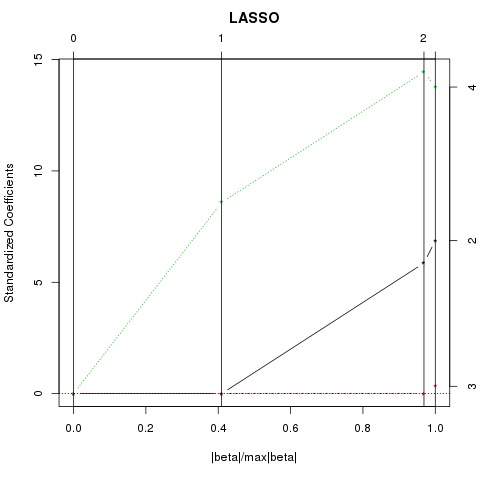
\includegraphics[scale=0.60]{a_regularization/lasso_result.png}
\caption{Graph of solution paths for LASSO.}
\label{plot:lasso_result}
\end{figure}

% other packages
Other packages provide implementations of the Lasso penalty method.
The \texttt{glmnet} package provides the LASSO and Elastic Net regularization for Generalized Linear Models (GLMs) using Coordinate Descent \cite{Friedman2011}.
The \texttt{grplasso} package provides an the Group Lasso penalty method for fitting models \cite{Meier2009}.
The \texttt{grpreg} package provides lasso regularization with grouped covariates \cite{Brehen2011}.

% lmmlasso package?!?
% penalized package

% References: Deeper understanding
% The references element description includes a listing of both primary sources of information about the technique as well as useful introductory sources for novices to gain a deeper understanding of the theory and application of the technique. The description consists of hand-selected reference material including books, peer reviewed conference papers, journal articles, and potentially websites. A bullet-pointed structure is suggested.
\subsection{References}
% What are the primary sources for a technique?
% What are the suggested reference sources for learning more about a technique?

% primary sources
\subsubsection{Primary Sources}
% primary
The LASSO method was described in detail by Tibshirani who also provided a Bayes model for the LASSO, simulation studies and extensions to generalization regression and other problems \cite{Tibshirani1996}. Tibshirani attributes the motivation the LASSO to Breiman's Non-negative Garrotte regression method \cite{Breiman1993} (later published \cite{Breiman1995}).
The LASSO is equivalent to Basis Pursuit from the field of Signal Processing \cite{Chen1998}.

% more info
\subsubsection{More Information}
The focus of the research into the LASSO is on efficient algorithms for solving the objective function.
% lars
Efron et~al.\ developed an efficient algorithm for computing the entire regularization path for the LASSO called Least Angle Regression (LARS) \cite{Efron2002}. LARS is based on the Homotopy method described by Osborne et~al.\ \cite{Osborne2000}. LARS has the same computational cost as the full least-squares fit on the data, exploiting the fact the coefficient profiles are piecewise linear.

% coordinate descent
Many solutions to the LASSO method have been proposed that optimize one parameter (coordinate) at a time, so called path-wise or coordinate-wise optimization methods. Early attempts were made by Fu in an investigation of cyclic coordinate descent for $L_2$ regression \cite{Fu1998} and Daubechies et~al.\ \cite{Daubechies2004}. The approach was re-discovered and promoted as an competitive and simpler alternative to LARS by Friedman et~al.\ for LASSO and related regularization methods with linearly-separable coefficients \cite{Friedman2007}. Wu and Lange provide a in-depth study of coordinate descent algorithms for LASSO penalized regression \cite{Wu2008}.

% extensions
There are many extensions to the LASSO method.
Graphical LASSO is an application of the method to undirected graphical models \cite{Friedman2008a}.
Fused LASSO the penalizes the $L_1$-norm of both the coefficients and their successive differences suitable for problems with features that can be ordered \cite{Tibshirani2005}.
Group LASSO \cite{Yuan2006} and Blockwise Sparse Regression (BSR) \cite{Kim2006} are extensions of the LASSO method for finding sparse groups (block-wise sparsity) of variables.
Zou and Hastie describe the Elastic Net which combines the $L_1$-penalty of LASSO with the $L_2$-penalty of Ridge Regression and provide a LARS-based solution \cite{Zou2005}.


% END\putbib\end{bibunit}
\newpage\begin{bibunit}% The Clever Algorithms Project: http://www.CleverAlgorithms.com
% (c) Copyright 2011 Jason Brownlee. Some Rights Reserved. 
% This work is licensed under a Creative Commons Attribution-Noncommercial-Share Alike 2.5 Australia License.

% Name
% The algorithm name defines the canonical name used to refer to the technique, in addition to common aliases, abbreviations, and acronyms. The name is used in terms of the heading and sub-headings of an algorithm description.
\section{Elastic Net} 
\label{sec:elasticnet}
\index{Elastic-Net}

% other names
% What is the canonical name and common aliases for a technique?
% What are the common abbreviations and acronyms for a technique?
\emph{Elastic Net, Elastic-Net, Na\"ive Elastic Net}

% Taxonomy: Lineage and locality
% The algorithm taxonomy defines where a techniques fits into the field, both the specific subfields of Computational Intelligence and Biologically Inspired Computation as well as the broader field of Artificial Intelligence. The taxonomy also provides a context for determining the relation- ships between algorithms. The taxonomy may be described in terms of a series of relationship statements or pictorially as a venn diagram or a graph with hierarchical structure.
\subsection{Taxonomy}
% To what fields of study does a technique belong?
Elastic Net is a Regularization method for Multiple Linear Regression models, and can be generalized to other machine learning methods.
% What are the closely related approaches to a technique?
It is related to other Regularization methods such as LASSO and Ridge Regression.

% Strategy: Problem solving plan
% The strategy is an abstract description of the computational model. The strategy describes the information processing actions a technique shall take in order to achieve an objective. The strategy provides a logical separation between a computational realization (procedure) and a analogous system (metaphor). A given problem solving strategy may be realized as one of a number specific algorithms or problem solving systems. The strategy description is textual using information processing and algorithmic terminology.
\subsection{Strategy}
% What is the information processing objective of a technique?
The information processing objective of the Elastic Net is to promote a parsimonious model.
% What is a techniques plan of action?
This is achieved by adding a penalty term that is a sum of the term used for Ridge Regression (squared sum of the coefficient values or $L_2$-norm) and the term used in the LASSO method (sum of absolute coefficient values or the $L_1$-norm). This penalty term is added to the models cost function with a penalty weight parameter ($\alpha$) and a shrinkage parameter $t$ that imposes a linear constraint on the term. 
It was proposed to address the limitations in the LASSO when Ridge Regression was demonstrated to perform better. 

Na\"ive Elastic Net is a two-stage procedure, first for each 

% optimization solutions
A modification of the Least Angle Regression (LARS) algorithm was proposed to solve the Elastic Net objective function called Least Angle Regression Elastic Net (LARS-EN).

% Heuristics: Usage guidelines
% The heuristics element describe the commonsense, best practice, and demonstrated rules for applying and configuring a parameterized algorithm. The heuristics relate to the technical details of the techniques procedure and data structures for general classes of application (neither specific implementations not specific problem instances). The heuristics are described textually, such as a series of guidelines in a bullet-point structure.
\subsection{Heuristics}
% What are the suggested configurations for a technique?
% What are the guidelines for the application of a technique to a problem instance?

\begin{itemize}
	\item It is expected to be useful in problems with a large number of predictors $p$ and a smaller number of observations $n$, $p>n$ problems.
	\item When the penalty weighting is 1 ($\alpha=1$), Na\"ive Elastic Net behaves like Ridge Regression. $\alpha$ is typically $\in \{0.1)$
	\item It can perform shrinkage of coefficients and variable selection simultaneously in the same way that the LASSO can.
	\item It has been demonstrated to outperform the LASSO while achieving a similarly sparse models.
	\item It encourages a grouping effect, where strongly correlated predictors tend to be in or out of the model together, a feature that had to be explicitly added to the LASSO in Group LASSO.
\end{itemize}

% sample script in R
\subsection{Code Listing}
% listing
Listing~\ref{glmnet_elastic_net} provides a code listing Elastic Net method in R.
% algorithm and package
The example uses the \texttt{glmnet()} function in the \texttt{glmnet} core package. The demonstration provides an example of a logistic regression with regularization.
% problem

% TODO provide a better problem with real variable selection

\lstinputlisting[firstline=7,language=r,caption={Example of Elastic Net in R using the \texttt{glmnet()} function in the \texttt{glmnet} package.}, label=glmnet_elastic_net]{../src/algorithms/regularization/glmnet_elastic_net.R}

% other packages
% elasticnet package?


% References: Deeper understanding
% The references element description includes a listing of both primary sources of information about the technique as well as useful introductory sources for novices to gain a deeper understanding of the theory and application of the technique. The description consists of hand-selected reference material including books, peer reviewed conference papers, journal articles, and potentially websites. A bullet-pointed structure is suggested.
\subsection{References}
% What are the primary sources for a technique?
% What are the suggested reference sources for learning more about a technique?

% primary sources
\subsubsection{Primary Sources}
% seminal
The Elastic-Net was described by Zou and Hastie to address short-comings in LASSO by combining the penalty functions of Ridge Regression and the LASSO \cite{Zou2005}. Both a Na\"ive Elastic Net and the Elastic Net method proper were described as was a solution to the objective function called Least Angle Regression Elastic Net (LARS-EN).

% more info
\subsubsection{More Information}



% END
\putbib\end{bibunit}
\newpage\begin{bibunit}% The Clever Algorithms Project: http://www.CleverAlgorithms.com
% (c) Copyright 2013 Jason Brownlee. Some Rights Reserved. 
% This work is licensed under a Creative Commons Attribution-Noncommercial-Share Alike 2.5 Australia License.


% Name
% The algorithm name defines the canonical name used to refer to the technique, in addition to common aliases, abbreviations, and acronyms. The name is used in terms of the heading and sub-headings of an algorithm description.
\section{Ridge Regression} 
\label{sec:ridge}
\index{Ridge Regression}
\index{Tikhonov Regularization}
\index{Tikhonov-Miller Method}
\index{Phillips-Twomey Method}
\index{Constrained Linear Inversion}
\index{Linear Regularization}
\index{Penalized $L_2$ Regression}
\index{$L_2$-norm Penalty}

% other names
% What is the canonical name and common aliases for a technique?
% What are the common abbreviations and acronyms for a technique?
\emph{Ridge Regression, Tikhonov Regularization, Tikhonov-Miller Method, Phillips-Twomey Method, Constrained Linear Inversion, Linear Regularization, Penalized $L_2$ Regression}

% Taxonomy: Lineage and locality
% The algorithm taxonomy defines where a techniques fits into the field, both the specific subfields of Computational Intelligence and Biologically Inspired Computation as well as the broader field of Artificial Intelligence. The taxonomy also provides a context for determining the relation- ships between algorithms. The taxonomy may be described in terms of a series of relationship statements or pictorially as a venn diagram or a graph with hierarchical structure.
\subsection{Taxonomy}
% To what fields of study does a technique belong?
Ridge Regression is a Regularization method for Multiple Linear Regression models.
% What are the closely related approaches to a technique?
Ridge Regression is related to other Regularized Regression models such as the LASSO and Elastic Net.
The general method of penalizing a model based on the sum of squared parameters is related to Weight Decay in the training of Artificial Neural Networks.

% Strategy: Problem solving plan
% The strategy is an abstract description of the computational model. The strategy describes the information processing actions a technique shall take in order to achieve an objective. The strategy provides a logical separation between a computational realization (procedure) and a analogous system (metaphor). A given problem solving strategy may be realized as one of a number specific algorithms or problem solving systems. The strategy description is textual using information processing and algorithmic terminology.
\subsection{Strategy}
% What is the information processing objective of a technique?
The information processing objective of Ridge Regression is to reduce or shrink the magnitude of the coefficients in a regression model.
% What is a techniques plan of action?
This is achieved by penalizing models based on the sum of the squared coefficients called an $L_2$ penalty or the $L_2$ norm. This term is added to the regression equation during the preparation of the model and is weighted by a complexity parameter ($\lambda$) that controls the amount of shrinkage of the coefficients. 
The effect is that coefficients of a regression model are shrunk towards zero during the training of the model. The intercept is not penalized.

% Heuristics: Usage guidelines
% The heuristics element describe the commonsense, best practice, and demonstrated rules for applying and configuring a parameterized algorithm. The heuristics relate to the technical details of the techniques procedure and data structures for general classes of application (neither specific implementations not specific problem instances). The heuristics are described textually, such as a series of guidelines in a bullet-point structure.
\subsection{Heuristics}
% What are the suggested configurations for a technique?
% What are the guidelines for the application of a technique to a problem instance?

\begin{itemize}
	\item It commonly results in a model with a better bias-variance trade-off than Ordinary Least Squares.
	\item The ridge constant $\lambda$ is typically selected in the range $[0,1]$, where $\lambda=0$ corresponds to an Ordinary Least Squares regression.
	\item Unlike other selection methods, Ridge Regression does not drop coefficients, all model parameters are maintained at the end of the process providing shrinkage but not selection of parameters.
	\item Inputs are commonly standardized before training the model as models are not equivalent under scaling.
	\item Cross-validation is commonly used to assess the model and model selection or stopping criteria.
	\item It is suited for problems where there are more predictors $p$ than there are observations $n$, $p>n$ problems.
\end{itemize}

% sample script in R
\subsection{Code Listing}
% listing
Listing~\ref{mass_ridge_regression} provides a code listing of the Ridge Regression method in R.
% algorithm and package
The example uses the \texttt{lm.ridge()} function in the \texttt{MASS} core package which is responsible for fitting linear models using Ridge Regression. The example trials a sequence of lambda values then uses the model with the best lambda value for prediction. Figure~\ref{plot:ridge_regression_result} provides a plot of the final coefficient values of each model for the given lambda values. For more information on this library type: \texttt{library(help="MASS")}, and for more information on the function type: \texttt{?lm.ridge}.

% problem
The test problem is a four-dimensional dataset of 100 samples, where \texttt{x3} and \texttt{y} are dependent on \texttt{x1} and \texttt{x1} and \texttt{x2} are independent variables. The problem is ill defined as \texttt{y} given \texttt{x1, x2, x3}. The model is expected to reduce the contribution of \texttt{x2} and \texttt{x3} toward zero leaving \texttt{y} given \texttt{x1}.

\lstinputlisting[firstline=7,language=r,caption={Example of Ridge Regression in R using the \texttt{lm.ridge()} function in the \texttt{MASS} package.}, label=mass_ridge_regression]{../src/algorithms/regularization/mass_ridge_regression.R}

\begin{figure}[htp]
\centering
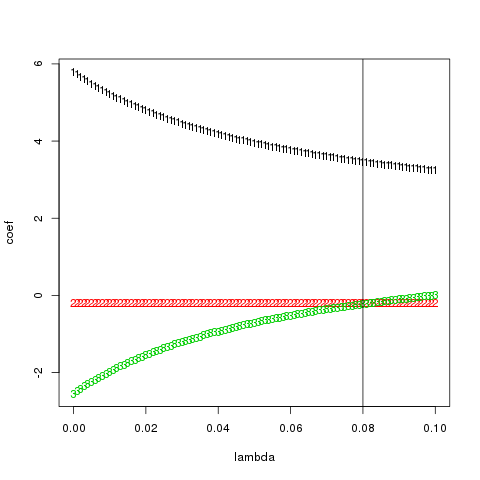
\includegraphics[scale=0.70]{book/a_regularization/ridge_regression_result.png}
\caption{Plot of the final coefficient values of each model for the given lambda values. The numbers reflect the \texttt{x} variables 1, 2 and 3. The line shows a selected lambda value.}
\label{plot:ridge_regression_result}
\end{figure}

% other packages ?
Other packages that provide an implementation of Ridge Regression include \texttt{parcor}.
% penalized package

% References: Deeper understanding
% The references element description includes a listing of both primary sources of information about the technique as well as useful introductory sources for novices to gain a deeper understanding of the theory and application of the technique. The description consists of hand-selected reference material including books, peer reviewed conference papers, journal articles, and potentially websites. A bullet-pointed structure is suggested.
\subsection{References}
% What are the primary sources for a technique?
% What are the suggested reference sources for learning more about a technique?

% primary sources
\subsubsection{Primary Sources}
% seminal
The method was originally described by Tikhonov \cite{Tikhonov1943, Tikhonov1963} (Russian), who later published a full account of the method as a book \cite{Tikhonov1977}.
% others
Phillips independently described the method \cite{Phillips1962}. Hoerl was first to use the term `Ridge Regression' which was adopted in the field of Statistics for $p>n$ problems \cite{Hoerl1962, Hoerl1970, Hoerl1970a}.

% more info
\subsubsection{More Information}
Hastie et~al.\ provide a gentle introduction to the method from the perspective of linear regression (\cite{Hastie2009}, page 61).
% applied
Press et~al.\ provide an introduction to Ridge Regression with examples in the C programming language \cite{Press2007} (Chapter 19).
Faraway provides an introduction to Ridge Regression with examples in R \cite{Faraway2002}.

% END
\putbib\end{bibunit}




	% correct handling of the index (new odd page)
  \cleardoublepage
  \phantomsection
	\addcontentsline{toc}{part}{Index}
	{\footnotesize \printindex}	
	
	% blank page
	\blanknonumber\cleardoublepage
	
\end{document}
